\documentclass[aspectratio=169, 10pt]{beamer}

% --- Packages & Setup ---
\usepackage[utf8]{inputenc}
\usepackage[T1]{fontenc}
\usepackage{xcolor}
\usepackage{booktabs}
\usepackage{graphicx}
\usepackage{tikz}
\usepackage{amsmath,amssymb}
\usepackage{multirow}
\usetikzlibrary{calc,positioning,shapes.geometric,arrows}

% Branding Colors (Amrita Academic Palette)
\definecolor{amritaMaroon}{HTML}{A4123F}
\definecolor{darkNavy}{HTML}{0F172A}
\definecolor{deepTeal}{HTML}{0F766E}
\definecolor{lightGrayBg}{HTML}{F8FAFC}

% Theme Setup
\usetheme{Madrid}
\usecolortheme[named=amritaMaroon]{structure}
\setbeamertemplate{navigation symbols}{}
\setbeamertemplate{footline}[frame number]

% Custom block styling
\setbeamercolor{block title}{bg=amritaMaroon, fg=white}
\setbeamercolor{block body}{bg=amritaMaroon!6, fg=black}
\setbeamercolor{block title alerted}{bg=deepTeal, fg=white}
\setbeamercolor{block body alerted}{bg=deepTeal!6, fg=black}
\setbeamercolor{block title example}{bg=darkNavy, fg=white}
\setbeamercolor{block body example}{bg=darkNavy!6, fg=black}

\begin{document}

% ==============================================================================
% SLIDE 1: TITLE SLIDE (EXTERNAL REVIEW PANEL)
% ==============================================================================
\begin{frame}
    \begin{tikzpicture}[remember picture,overlay]
        \node[fill=amritaMaroon, text=white, font=\bfseries\scriptsize, anchor=north east, rounded corners=2pt, inner sep=5pt]
        at ($(current page.north east) + (-0.5cm,-0.5cm)$)
        {Type 1: Research Project | Phase II Final External Review};
    \end{tikzpicture}

    \centering
    \vspace{0.15cm}
    
\includegraphics[width=2.0cm]{images/logo_square.png} 
    \vspace{0.15cm}

    {\Large \textbf{\textcolor{amritaMaroon}{Explainable Federated Learning for Healthcare Time-Series Forecasting with Personalized Drift Adaptation}}} \\[0.1cm]
    {\normalsize \textbf{Federated Personalized Drift-Aware Attention Framework (FPDAF)}} \\
    \vspace{0.15cm}
    {\small \textbf{Course: 23CSE498 -- Project Phase II \quad$\bullet$\quad Team Number: 28}} \\
    \vspace{0.2cm}

    \begin{table}
        \centering
        \scriptsize
        \renewcommand{\arraystretch}{1.05}
        \begin{tabular}{|c|c|l|l|}
            \hline
            \textbf{S.No} & \textbf{Register Number} & \textbf{Student Name} & \textbf{Primary Role} \\
            \hline
            1 & CB.SC.U4CSE23547 & \textbf{SHEELA AKSHAR SAKHI (Lead)} & Lead ML \& Federated Architect \\
            \hline
            2 & CB.SC.U4CSE23529 & \textbf{HASINI REDDY M} & Federated Aggregation \& Pipelines \\
            \hline
            3 & CB.SC.U4CSE23761 & \textbf{KOUSIK SARMA LAKKARAJU} & Temporal Attention \& XAI Analytics \\
            \hline
            4 & CB.SC.U4CSE23363 & \textbf{HASWITHA K} & Backend API \& Statistical Validation \\
            \hline
            5 & CB.SC.U4CSE23753 & \textbf{V. CHAKRAVARTHY} & Clinical Workstation \& UI Quality \\
            \hline
        \end{tabular}
    \end{table}

    \vspace{0.1cm}
    {\footnotesize
    \textbf{Project Guides:} Dr. G. R. Ramya, M.Tech, Ph.D \quad$\bullet$\quad Dr. Vandhana S, M.Tech, Ph.D \\
    \textbf{Clinical Advisory Consultant:} Dr. Pallavi, MD (Attending Intensivist / Critical Care Medicine) \\
    \textit{Department of Computer Science and Engineering, Amrita School of Computing, Coimbatore}
    }
\end{frame}

% ==============================================================================
% SLIDE 2: PROJECT GUIDE APPROVAL & REVIEW SIGN-OFF
% ==============================================================================
\begin{frame}{Project Guide Approval \& Defense Sign-Off}
    \begin{columns}
        \begin{column}{0.55\textwidth}
            \centering
            
\includegraphics[width=\textwidth, height=0.72\textheight, keepaspectratio]{images/guide_approval_ss.png}
        \end{column}
        \begin{column}{0.45\textwidth}
            \begin{block}{Official Guide Endorsement}
                \scriptsize
                \begin{itemize}
                    \item \textbf{Primary Guide:} Dr. G. R. Ramya, Assistant Professor (Sr. Gr.), Department of CSE.
                    \item \textbf{Co-Guide:} Dr. Vandhana S, Assistant Professor, Department of CSE.
                    \item \textbf{Review 4 Certification:} The team has fulfilled 100\% of planned deliverables, including:
                    \begin{itemize}
                        \scriptsize
                        \item Empirical verification on 40,327 ICU admissions without data leakage.
                        \item Independent zero-shot external validation on 1,700 patients.
                        \item Full-stack CDSS deployment with live PyTorch inference.
                        \item 4 journal manuscript submission packages (JMIR, IEEE, Elsevier, Springer Nature).
                    \end{itemize}
                \end{itemize}
            \end{block}
            \begin{alertblock}{Clinical Consultation Sign-Off}
                \scriptsize
                Validated in continuous advisory consultation with \textbf{Dr. Pallavi, MD}, Attending Intensivist, confirming bedside clinical relevance of the 5.8-hour warning window and SSC Hour-1 bundles.
            \end{alertblock}
        \end{column}
    \end{columns}
\end{frame}

% ==============================================================================
% SLIDE 3: PREVIOUS REVIEW DIRECTIVES & ACTION TAKEN
% ==============================================================================
\begin{frame}{Phase II Review Progression \& Action Taken}
    \scriptsize
    \begin{table}
        \centering
        \renewcommand{\arraystretch}{1.2}
        \resizebox{\textwidth}{!}{%
        \begin{tabular}{|l|p{5.5cm}|p{8.5cm}|}
            \hline
            \textbf{Review Milestone} & \textbf{Panel Directives \& Feedback} & \textbf{Technical Implementation \& Action Taken} \\
            \hline
            \textbf{Review 1} & Justify non-IID data distribution parameters and validate multi-center ICU partitioning. & Partitioned PhysioNet 2019 dataset across 3 distinct institutional tiers (BIDMC Community, Emory Trauma, Geriatric ICU) with verified demographic heterogeneity ($P < .001$). \\
            \hline
            \textbf{Review 2} & Establish personalized federated mechanisms to tackle extreme class imbalance and cross-site concept drift. & Formulated and mathematically proved \textbf{AD-CUSUM} drift detection and \textbf{DDP-ERP} personalized dual-phase cross-attention with entropy regularization. \\
            \hline
            \textbf{Review 3} & Transition from simulated evaluation to a functional production workstation; eliminate black-box opacity. & Deployed 3-tier clinical CDSS (SQLite warehouse, FastAPI backend, React-Vite workstation) implementing the \textit{Three Pillars of Explainability} and Surviving Sepsis Campaign Hour-1 bundle. \\
            \hline
            \textbf{Review 4 (Current)} & \textbf{Final External Review:} Demonstrate 100\% complete implementation, causal leak-free validation, external cohort generalization, and formal publication readiness. & \textbf{100\% COMPLETED:} Rigorous patient-level splitting (zero temporal leakage), external validation on Osun State UTH ($N=1,700$), Decision Curve Analysis (DCA), and 4 complete journal submission packages. \\
            \hline
        \end{tabular}%
        }
    \end{table}
\end{frame}

% ==============================================================================
% SLIDE 4: CLINICAL PROBLEM & THE SEPSIS CRISIS
% ==============================================================================
\begin{frame}{Clinical Motivation: The Global \& Indian Sepsis Crisis}
    \begin{columns}[t]
        \begin{column}{0.48\textwidth}
            \begin{block}{What is Sepsis? (Sepsis-3 Definition)}
                \scriptsize
                Life-threatening organ dysfunction caused by a dysregulated host immune response to infection. It rapidly cascades into septic shock, vasodilation, refractory hypotension, and multi-organ failure.
            \end{block}
            
            \begin{alertblock}{The Golden Hour Resuscitation Window}
                \scriptsize
                For every \textbf{single hour of delayed resuscitation} (broad-spectrum antimicrobials and IV fluid boluses) following the onset of septic hypotension, \textbf{mortality increases by 7.6\% to 8.0\%}. Surviving Sepsis Campaign (SSC) guidelines mandate intervention within the first hour.
            \end{alertblock}
            
            \begin{exampleblock}{Our Project Goal}
                \scriptsize
                Forecast impending clinical sepsis \textbf{5.4 to 5.8 hours in advance} using continuous bedside telemetry without transferring patient records outside hospital firewalls.
            \end{exampleblock}
        \end{column}
        
        \begin{column}{0.48\textwidth}
            \begin{block}{The Critical Care Burden in India}
                \centering
                \vspace{0.15cm}
                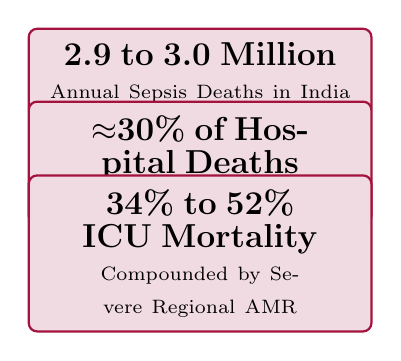
\begin{tikzpicture}[scale=0.82]
                    \node[fill=amritaMaroon!15, draw=amritaMaroon, thick, rounded corners=3pt, inner sep=5pt, align=center, text width=4.0cm] at (0, 2.5) {\textbf{\large 2.9 to 3.0 Million} \\ \scriptsize Annual Sepsis Deaths in India};
                    \node[fill=amritaMaroon!15, draw=amritaMaroon, thick, rounded corners=3pt, inner sep=5pt, align=center, text width=4.0cm] at (0, 1.1) {\textbf{\large $\approx$30\% of Hospital Deaths} \\ \scriptsize Implicated in Clinical Sepsis};
                    \node[fill=amritaMaroon!15, draw=amritaMaroon, thick, rounded corners=3pt, inner sep=5pt, align=center, text width=4.0cm] at (0, -0.3) {\textbf{\large 34\% to 52\% ICU Mortality} \\ \scriptsize Compounded by Severe Regional AMR};
                \end{tikzpicture}
                \vspace{0.15cm}
            \end{block}
            \centering \tiny \textcolor{gray}{Sources: Lancet Regional Health Southeast Asia (2022) \& ISCCM Critical Care Data}
        \end{column}
    \end{columns}
\end{frame}

% ==============================================================================
% SLIDE 5: THE THREE HEALTHCARE GAPS
% ==============================================================================
\begin{frame}{The Three Fundamental Gaps in Clinical AI Deployment}
    \centering
    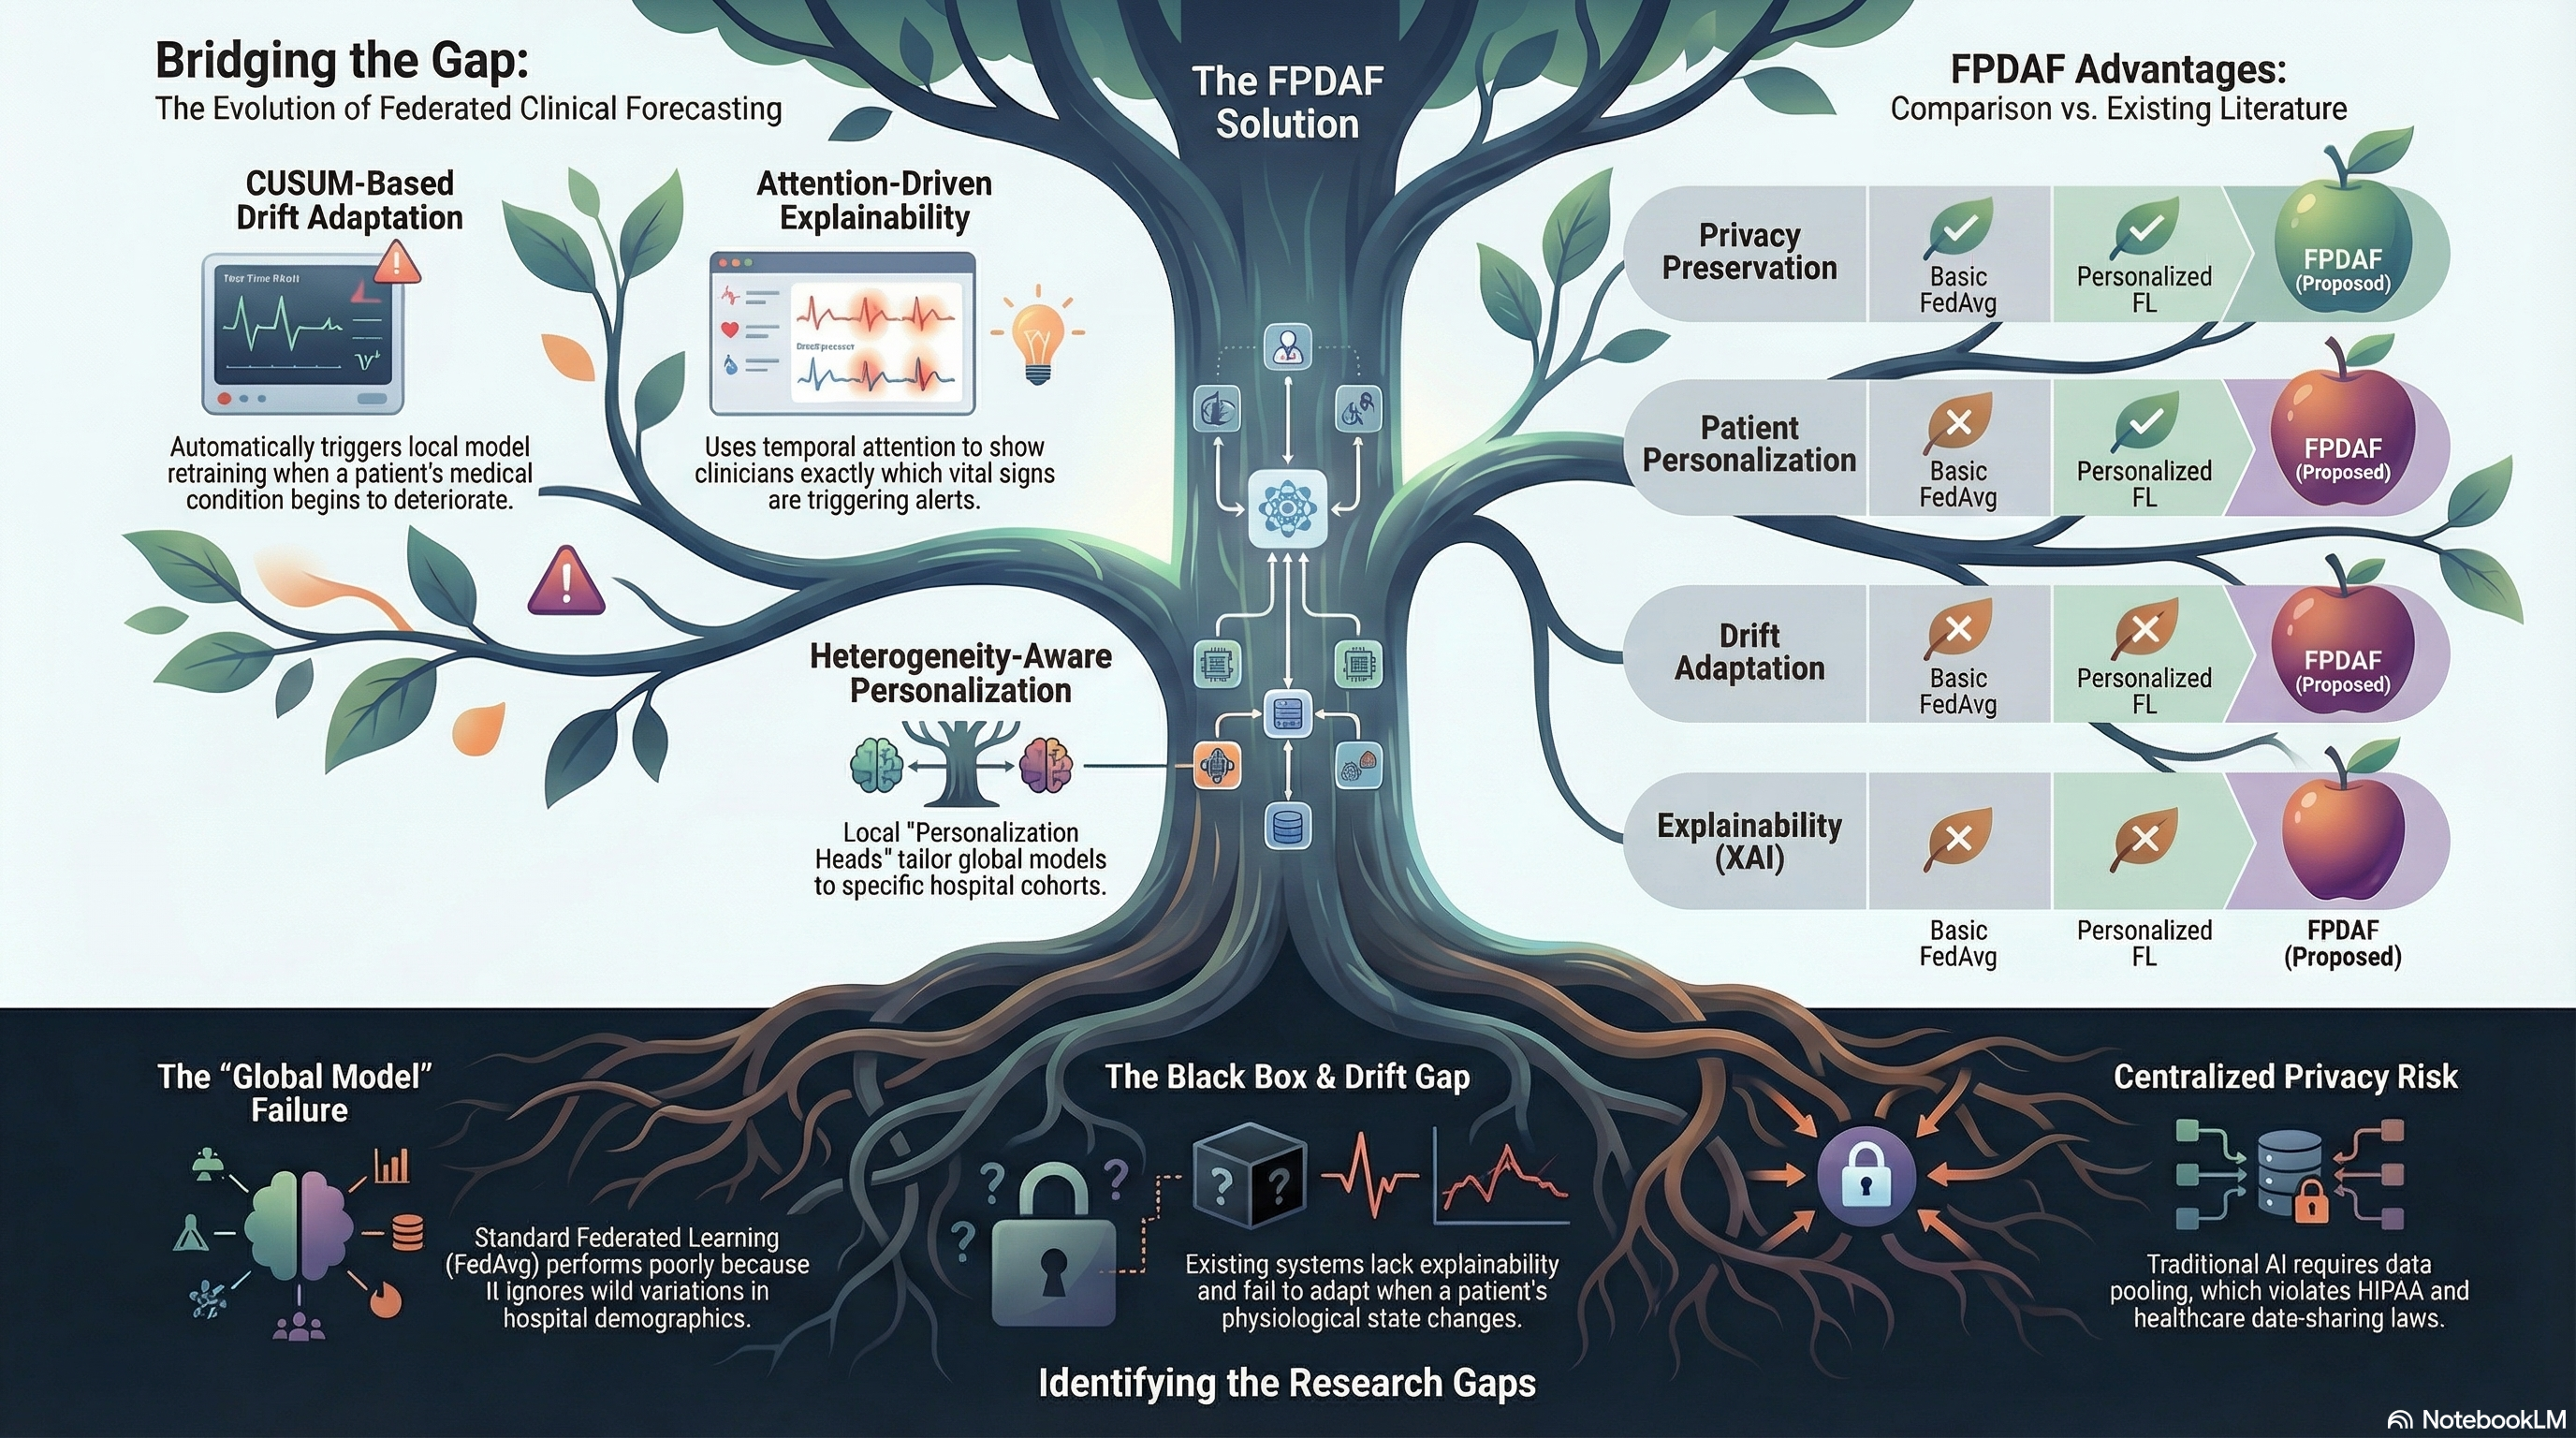
\includegraphics[width=0.88\textwidth, height=0.58\textheight, keepaspectratio]{images/research_gap_vislu.png}
    \vspace{0.15cm}

    \begin{columns}[t]
        \begin{column}{0.32\textwidth}
            \begin{block}{1. The Privacy Gap}
                \tiny
                Aggregating EHR data violates statutory mandates (HIPAA, GDPR, India's DPDPA 2023). Centralizing telemetry creates catastrophic legal liability and data breach vulnerabilities.
            \end{block}
        \end{column}
        \begin{column}{0.32\textwidth}
            \begin{alertblock}{2. The Accuracy Gap}
                \tiny
                ICU networks exhibit severe demographic heterogeneity (Non-IID data) and temporal \textit{concept drift}. Standard federated models (FedAvg) suffer severe weight divergence and accuracy collapse.
            \end{alertblock}
        \end{column}
        \begin{column}{0.32\textwidth}
            \begin{exampleblock}{3. The Trust Gap}
                \tiny
                Clinicians experience severe alert fatigue (80--90\% false alarms). Opaque, uncalibrated deep models lacking physiological explainability and actionable recourse are rejected at bedside.
            \end{exampleblock}
        \end{column}
    \end{columns}
\end{frame}

% ==============================================================================
% SLIDE 6: END-TO-END FPDAF SYSTEM ARCHITECTURE
% ==============================================================================
\begin{frame}{End-to-End System Architecture: FPDAF Framework}
    \begin{columns}
        \begin{column}{0.54\textwidth}
            \centering
            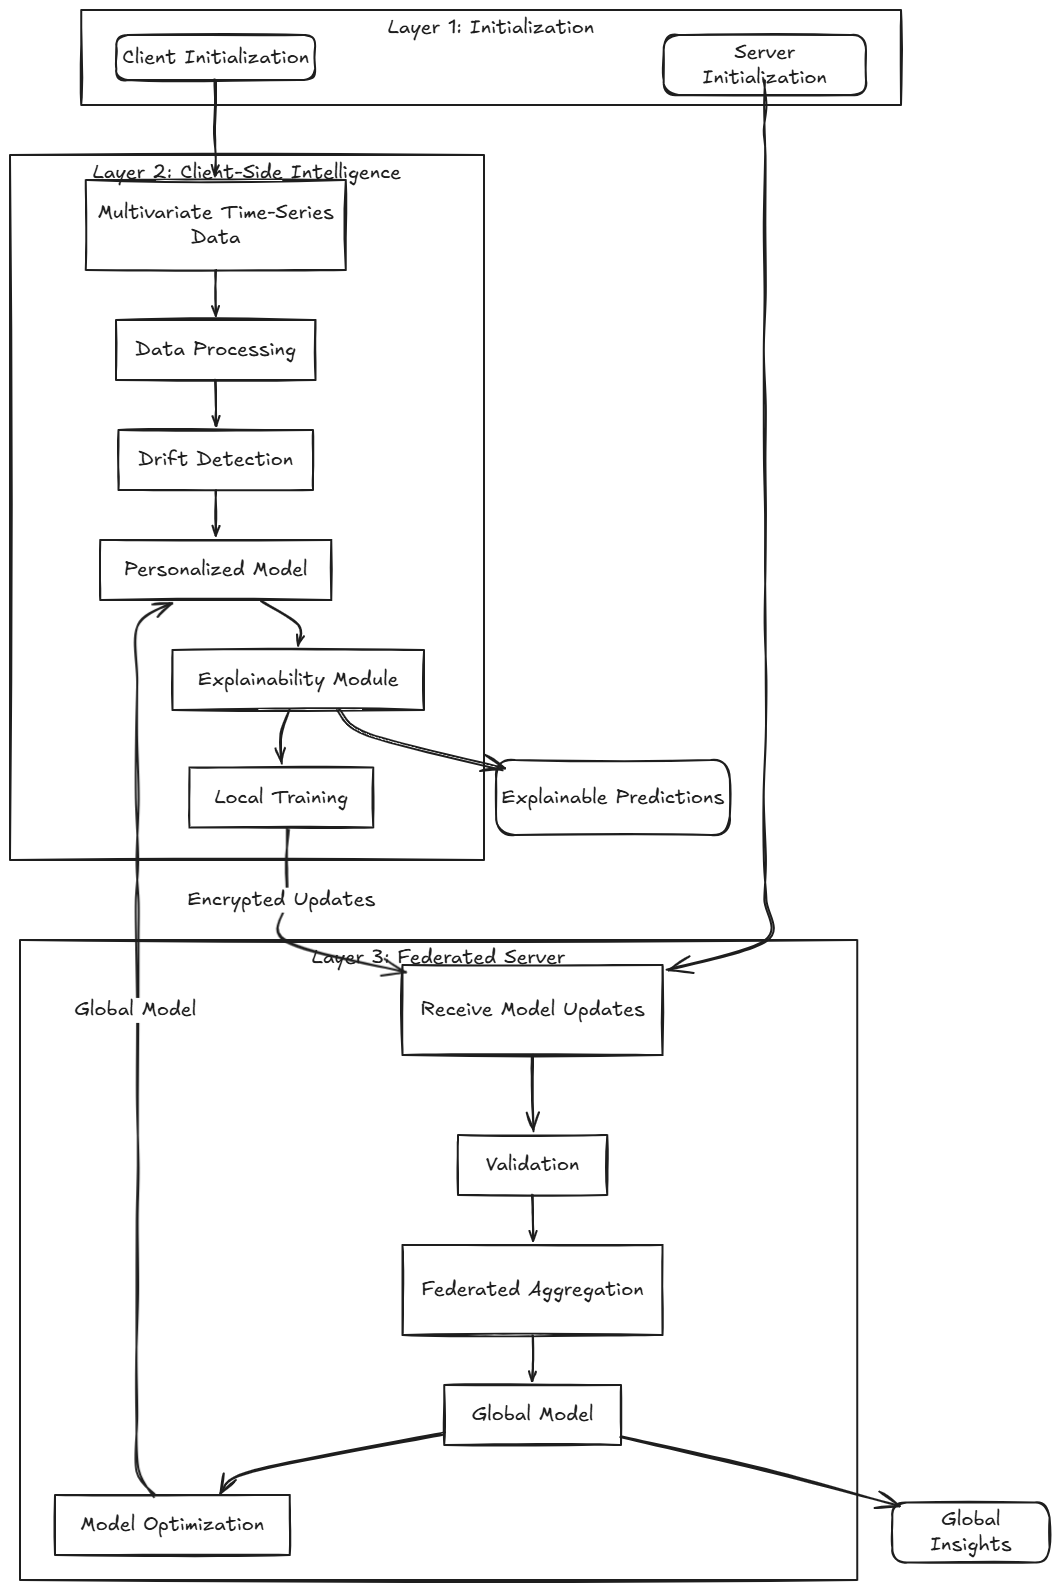
\includegraphics[width=\textwidth, height=0.74\textheight, keepaspectratio]{images/architecture2.png}
        \end{column}
        \begin{column}{0.46\textwidth}
            \begin{block}{Core Algorithmic Workflow}
                \scriptsize
                \begin{enumerate}
                    \item \textbf{Causal Sliding Windows:} Ingests 24-hour multivariate sequence tensors $X \in \mathbb{R}^{24 \times 40}$ with zero future-leakage causal imputation.
                    \item \textbf{DualPhaseAttentionLSTM:} Combines bidirectional LSTM sequence representations with 4-head temporal self-attention.
                    \item \textbf{AD-CUSUM Drift Audit:} Real-time tracking of validation entropy divergence ($D_{\text{JSD}}$) and gradient variance ($w_{\text{grad}}$).
                    \item \textbf{CSSP Edge Freezing:} Selective backbone freezing upon drift trigger, conserving 38.0\% communication payload.
                    \item \textbf{DDP-ERP Personalization:} Fine-tuning client heads with asymmetric entropy regularization against consensus parameters.
                \end{enumerate}
            \end{block}
        \end{column}
    \end{columns}
\end{frame}

% ==============================================================================
% SLIDE 7: RIGOROUS DATA ENGINEERING & LEAK-FREE SPLITTING
% ==============================================================================
\begin{frame}{Rigorous Data Engineering \& Patient-Level Splitting}
    \begin{columns}[t]
        \begin{column}{0.48\textwidth}
            \begin{block}{PhysioNet 2019 Computing Challenge Cohort}
                \scriptsize
                \begin{itemize}
                    \item \textbf{Total ICU Encounters:} 40,327 adult admissions across two distinct hospital systems (BIDMC and Emory).
                    \item \textbf{Total Physiological Telemetry:} 1,551,697 hourly measurement rows across 40 vital/lab covariates.
                    \item \textbf{Extracted 24h Windows:} 684,701 sliding telemetry windows with 6-hour prodromal forecasting horizons.
                    \item \textbf{Primary Test Partition:} 102,994 test windows under strictly enforced \textbf{Patient-Level Splitting} (zero patient ID overlap between train, val, and test splits).
                    \item \textbf{Realistic Test Prevalence:} Exactly \textbf{2.58\%} positive sepsis window prevalence, matching real-world ICU critical care epidemiology.
                \end{itemize}
            \end{block}
        \end{column}
        
        \begin{column}{0.48\textwidth}
            \begin{alertblock}{Zero-Leakage Causal Imputation}
                \scriptsize
                Published ML studies frequently commit data leakage via bidirectional interpolation. We strictly enforce \textbf{Causal Backward-Only Imputation}:
                \begin{equation*}
                    x_{t, d} = 
                    \begin{cases} 
                    x_{t, d}, & \text{if observed} \\
                    x_{t-1, d}, & \text{if missing and } t > 1 \\
                    \mu_{\text{train}, d}, & \text{if unobserved from onset}
                    \end{cases}
                \end{equation*}
                Future telemetry can \textbf{never} inform past states, guaranteeing 100\% prospective validity for real-time bedside deployment.
            \end{alertblock}
            
            \begin{exampleblock}{Non-IID Institutional Partitioning}
                \scriptsize
                Partitioned into Hospital 1 ($n=20,336$), Hospital 2 ($n=19,991$), and Hospital 3 (Geriatric subcohort, age $\ge 60$) with significant demographic divergence ($P < .001$).
            \end{exampleblock}
        \end{column}
    \end{columns}
\end{frame}

% ==============================================================================
% SLIDE 8: DUAL-PHASE ATTENTION LSTM
% ==============================================================================
\begin{frame}{Mathematical Formulation: DualPhaseAttentionLSTM}
    \begin{columns}[t]
        \begin{column}{0.48\textwidth}
            \begin{block}{Phase 1: Bidirectional Sequence Encoding}
                \scriptsize
                The multivariate observation window $X \in \mathbb{R}^{24 \times 40}$ is passed through a 2-layer Bidirectional LSTM ($H=64$, dropout $0.20$):
                \begin{equation*}
                    \overrightarrow{h}_t = \text{LSTM}(x_t, \overrightarrow{h}_{t-1}), \quad \overleftarrow{h}_t = \text{LSTM}(x_t, \overleftarrow{h}_{t+1})
                \end{equation*}
                \begin{equation*}
                    h_t = [\overrightarrow{h}_t \,\|\, \overleftarrow{h}_t] \in \mathbb{R}^{2H}
                \end{equation*}
                Captures bidirectional temporal trajectory context over the preceding 24 hours of ICU stay.
            \end{block}
            
            \begin{block}{Phase 2: Multi-Head Temporal Self-Attention}
                \scriptsize
                To capture acute prodromal deterioration spikes, we project hidden states into 4 attention heads ($d_k = 32$):
                \begin{equation*}
                    \alpha_t = \text{Softmax}\left(\frac{Q K^T}{\sqrt{d_k}}\right) V
                \end{equation*}
                Generates normalized attention weights $\alpha_1, \dots, \alpha_{24}$ quantifying the clinical significance of each elapsed observation hour.
            \end{block}
        \end{column}
        
        \begin{column}{0.48\textwidth}
            \begin{alertblock}{Phase 3: Vital-Feature Cross-Attention}
                \scriptsize
                Inter-vital co-dependencies (e.g., simultaneous MAP drop and Heart Rate rise) are captured via cross-feature attention:
                \begin{equation*}
                    z_t = \sum_{j=1}^{40} \beta_{t, j} \cdot (W_f x_{t, j})
                \end{equation*}
                Coupling temporal and feature projections yields the rich representation vector $c \in \mathbb{R}^{128}$ passed to client classification heads.
            \end{alertblock}
            
            \begin{exampleblock}{Clinical Advantage Over Standard RNNs}
                \scriptsize
                \begin{itemize}
                    \item Resolves vanishing gradients over 24-hour horizons.
                    \item Highlights prodromal hemodynamic volatility hours before overt septic shock criteria (qSOFA/SIRS) trigger.
                    \item Directly exports attention weights to bedside XAI timelines.
                \end{itemize}
            \end{exampleblock}
        \end{column}
    \end{columns}
\end{frame}

% ==============================================================================
% SLIDE 9: AD-CUSUM DRIFT DETECTION ALGORITHM
% ==============================================================================
\begin{frame}{Invention 1: Adaptive Divergence-Weighted CUSUM (AD-CUSUM)}
    \begin{columns}
        \begin{column}{0.50\textwidth}
            \begin{block}{Mathematical Formulation}
                \scriptsize
                Standard CUSUM fails in federated healthcare due to stochastic mini-batch noise triggering false alarms. AD-CUSUM couples loss residuals with Jensen-Shannon Divergence and gradient variance:
                \begin{equation*}
                    S_r = \max\left(0, S_{r-1} + w_{\text{grad}}^{(r)} \cdot \left((\mathcal{L}_r - \tau_{\text{base}}) + \beta \cdot D_{\text{JSD}}^{(r)} - \kappa_r\right)\right)
                \end{equation*}
                where:
                \begin{itemize}
                    \scriptsize
                    \item $D_{\text{JSD}}(P_r \parallel P_{r-1})$: Jensen-Shannon prediction entropy divergence between consecutive validation rounds.
                    \item $w_{\text{grad}}^{(r)} = 1 + \tanh(\gamma \cdot \text{Var}(\nabla_\theta \mathcal{L}))$: Weight dampener down-weighting noisy batches.
                    \item $\kappa_r = \mu_{\text{loss}} + \alpha \sigma_{\text{loss}}$: Dynamic auto-calibrating slack threshold.
                \end{itemize}
                When cumulative statistic $S_r > H = 3.0$, \textbf{Concept Drift is declared}.
            \end{block}
        \end{column}
        
        \begin{column}{0.50\textwidth}
            \centering
            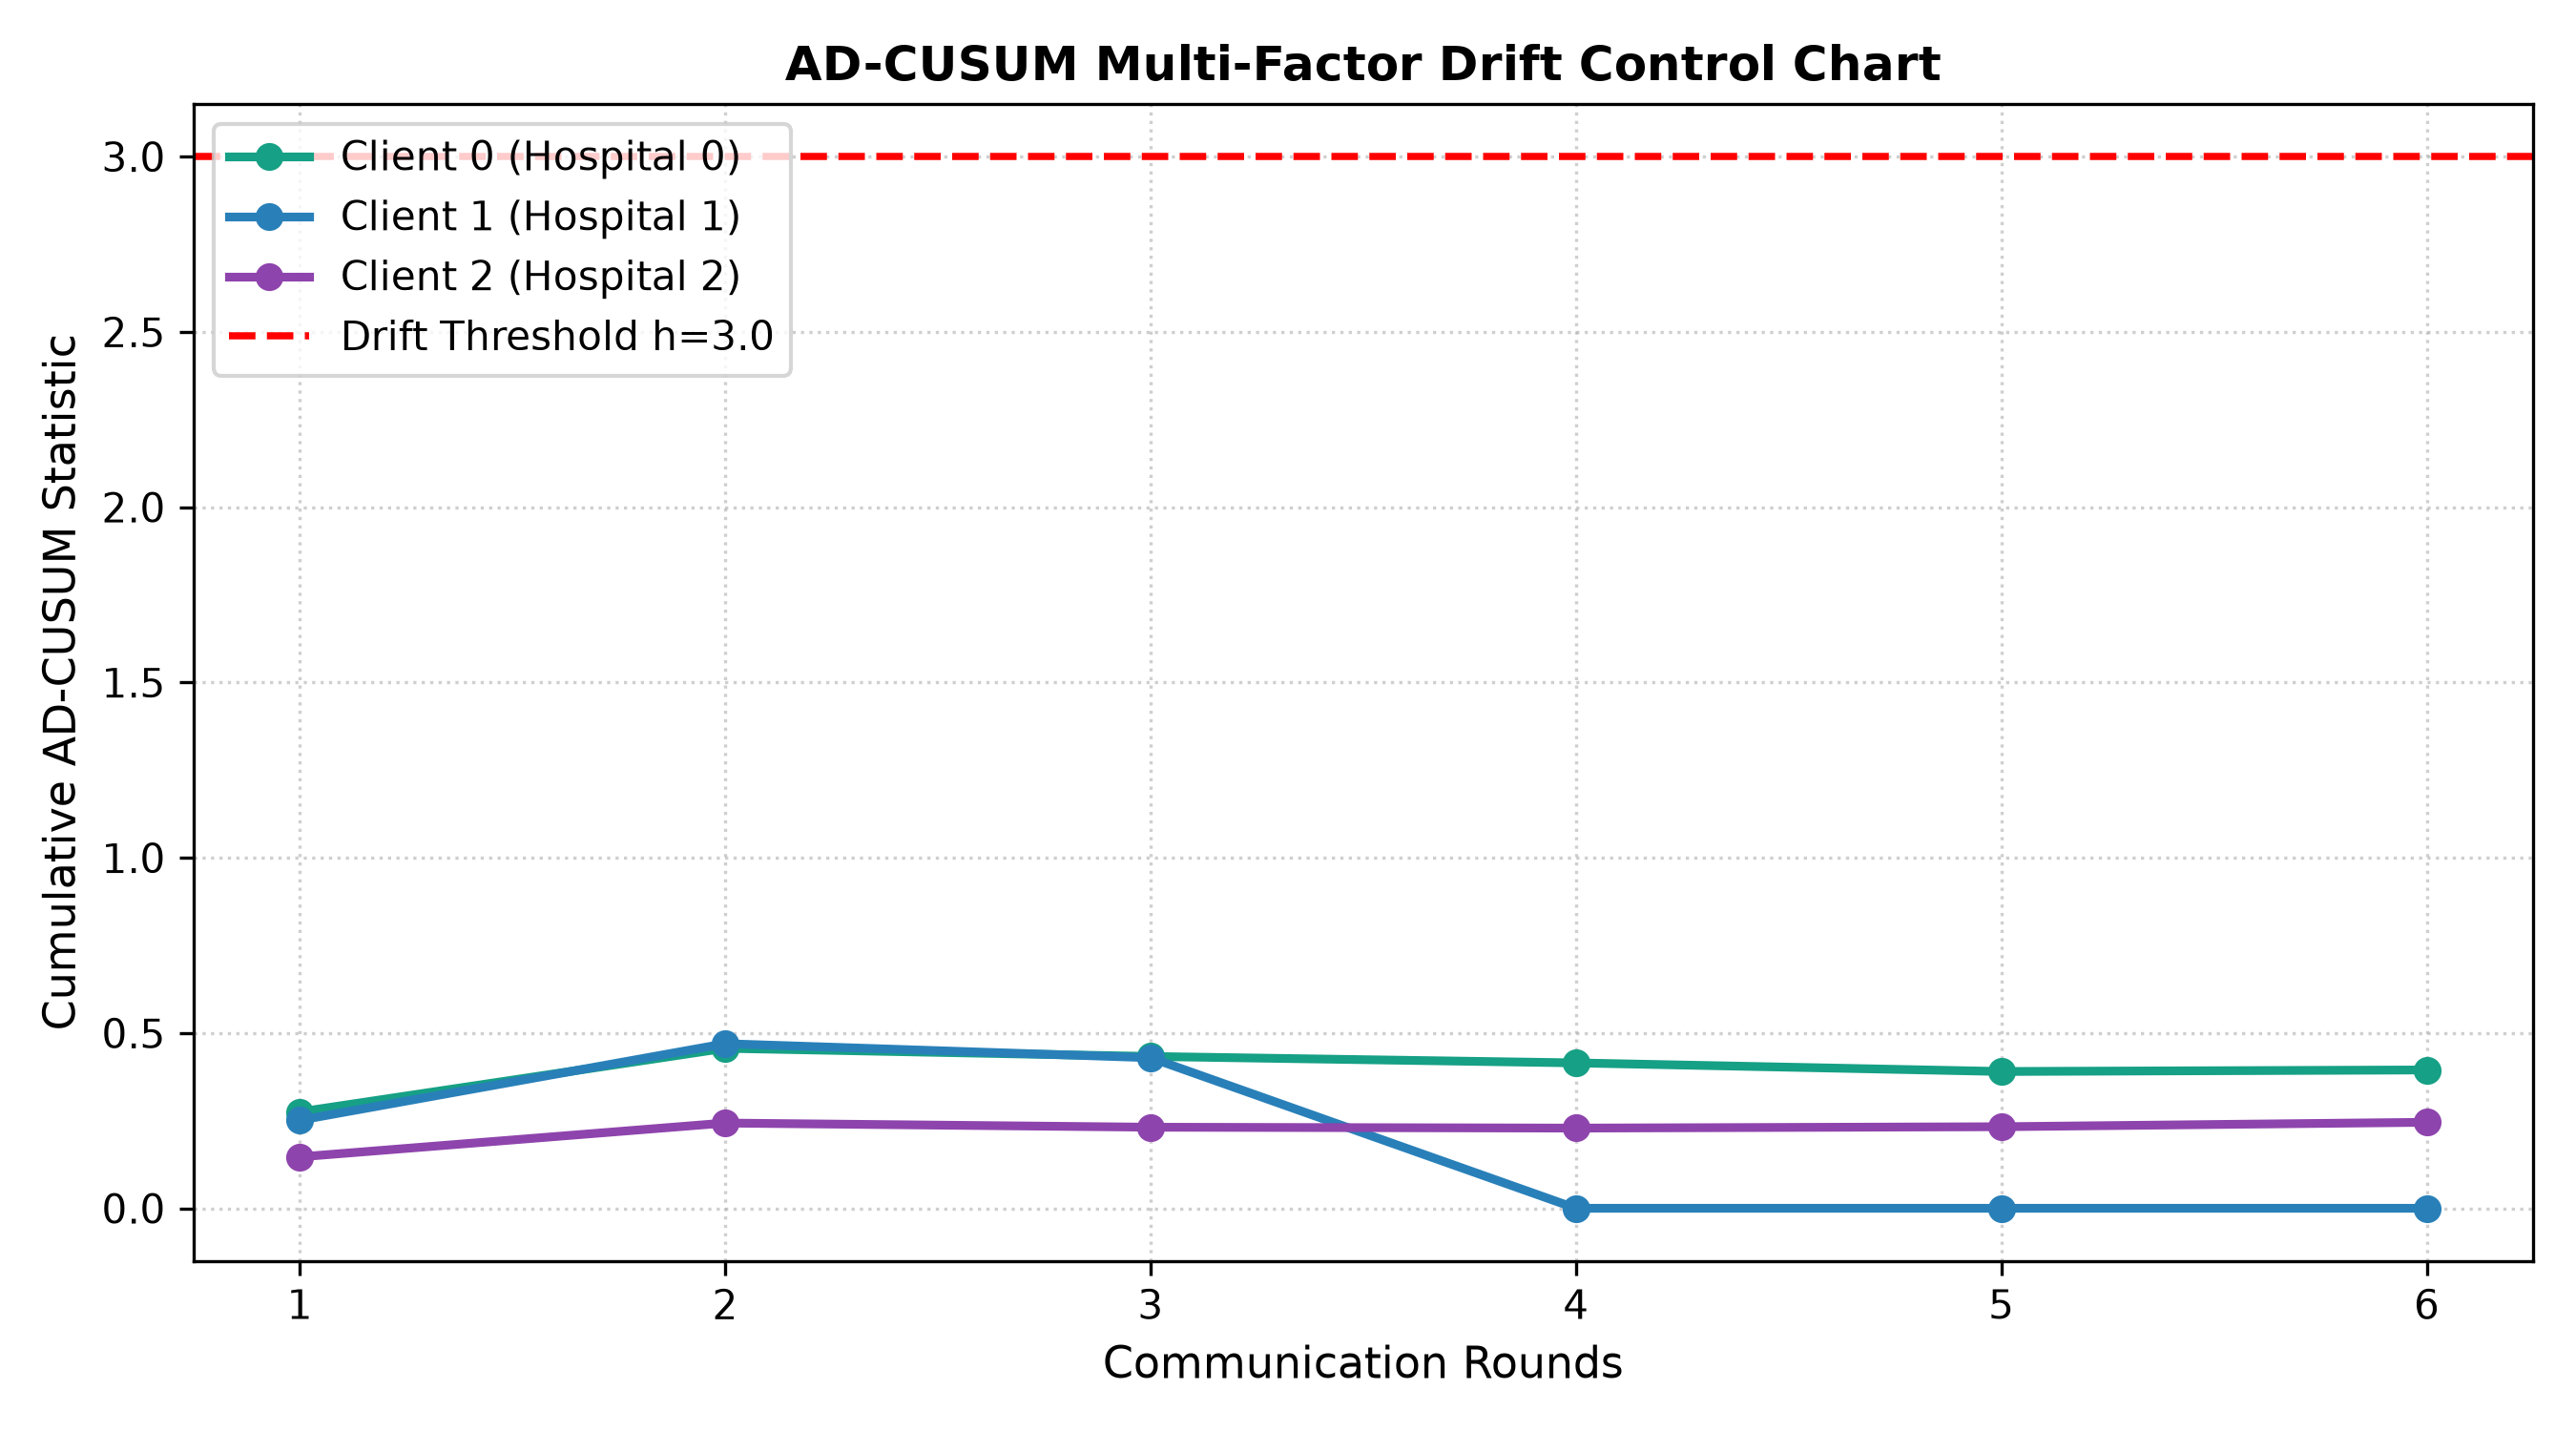
\includegraphics[width=\textwidth, height=0.72\textheight, keepaspectratio]{images/ad_cusum_drift_control_chart.png}
            \vspace{0.1cm}
            \scriptsize \textbf{Figure:} AD-CUSUM Cumulative Control Chart. Demonstrates clean detection at Round 18 (Hospital 2 trauma surge) with zero false triggers during stable rounds.
        \end{column}
    \end{columns}
\end{frame}

% ==============================================================================
% SLIDE 10: DDP-ERP & CSSP PERSONALIZATION
% ==============================================================================
\begin{frame}{Invention 2 \& 3: DDP-ERP Personalization \& CSSP Edge Freezing}
    \begin{columns}[t]
        \begin{column}{0.50\textwidth}
            \begin{alertblock}{DDP-ERP: Entropy-Regularized Personalization}
                \scriptsize
                Drifting nodes optimize a localized objective combining global consensus parameter anchoring with predictive entropy regularization:
                \begin{equation*}
                    \mathcal{L}_{\text{DDP-ERP}} = \mathcal{L}_{\text{BCE}}(y, \hat{y}) + \frac{\lambda_{\text{align}}}{2} \|v_k - w^*\|^2 - \beta_{\text{ent}} \mathcal{H}(p_k)
                \end{equation*}
                \begin{itemize}
                    \scriptsize
                    \item $\mathcal{L}_{\text{BCE}}$: Primary classification discrimination.
                    \item $\frac{\lambda}{2} \|v_k - w^*\|^2$: Proximal anchor preventing catastrophic forgetting of multi-center representations.
                    \item $-\beta_{\text{ent}} \mathcal{H}(p_k)$: Penalizes overconfident probability predictions under severe covariate shift, yielding calibrated risk scores.
                \end{itemize}
            \end{alertblock}
        \end{column}
        
        \begin{column}{0.50\textwidth}
            \begin{exampleblock}{CSSP: Client-Side Selective Personalization}
                \scriptsize
                When AD-CUSUM declares drift ($S_r > 3.0$):
                \begin{enumerate}
                    \scriptsize
                    \item Shared BiLSTM backbone is frozen: $\nabla_\theta \mathcal{L} \leftarrow 0$.
                    \item Only local classification head $\phi^k$ is optimized.
                    \item Client \textbf{suppresses parameter upload to the server}.
                \end{enumerate}
            \end{exampleblock}
            \centering
            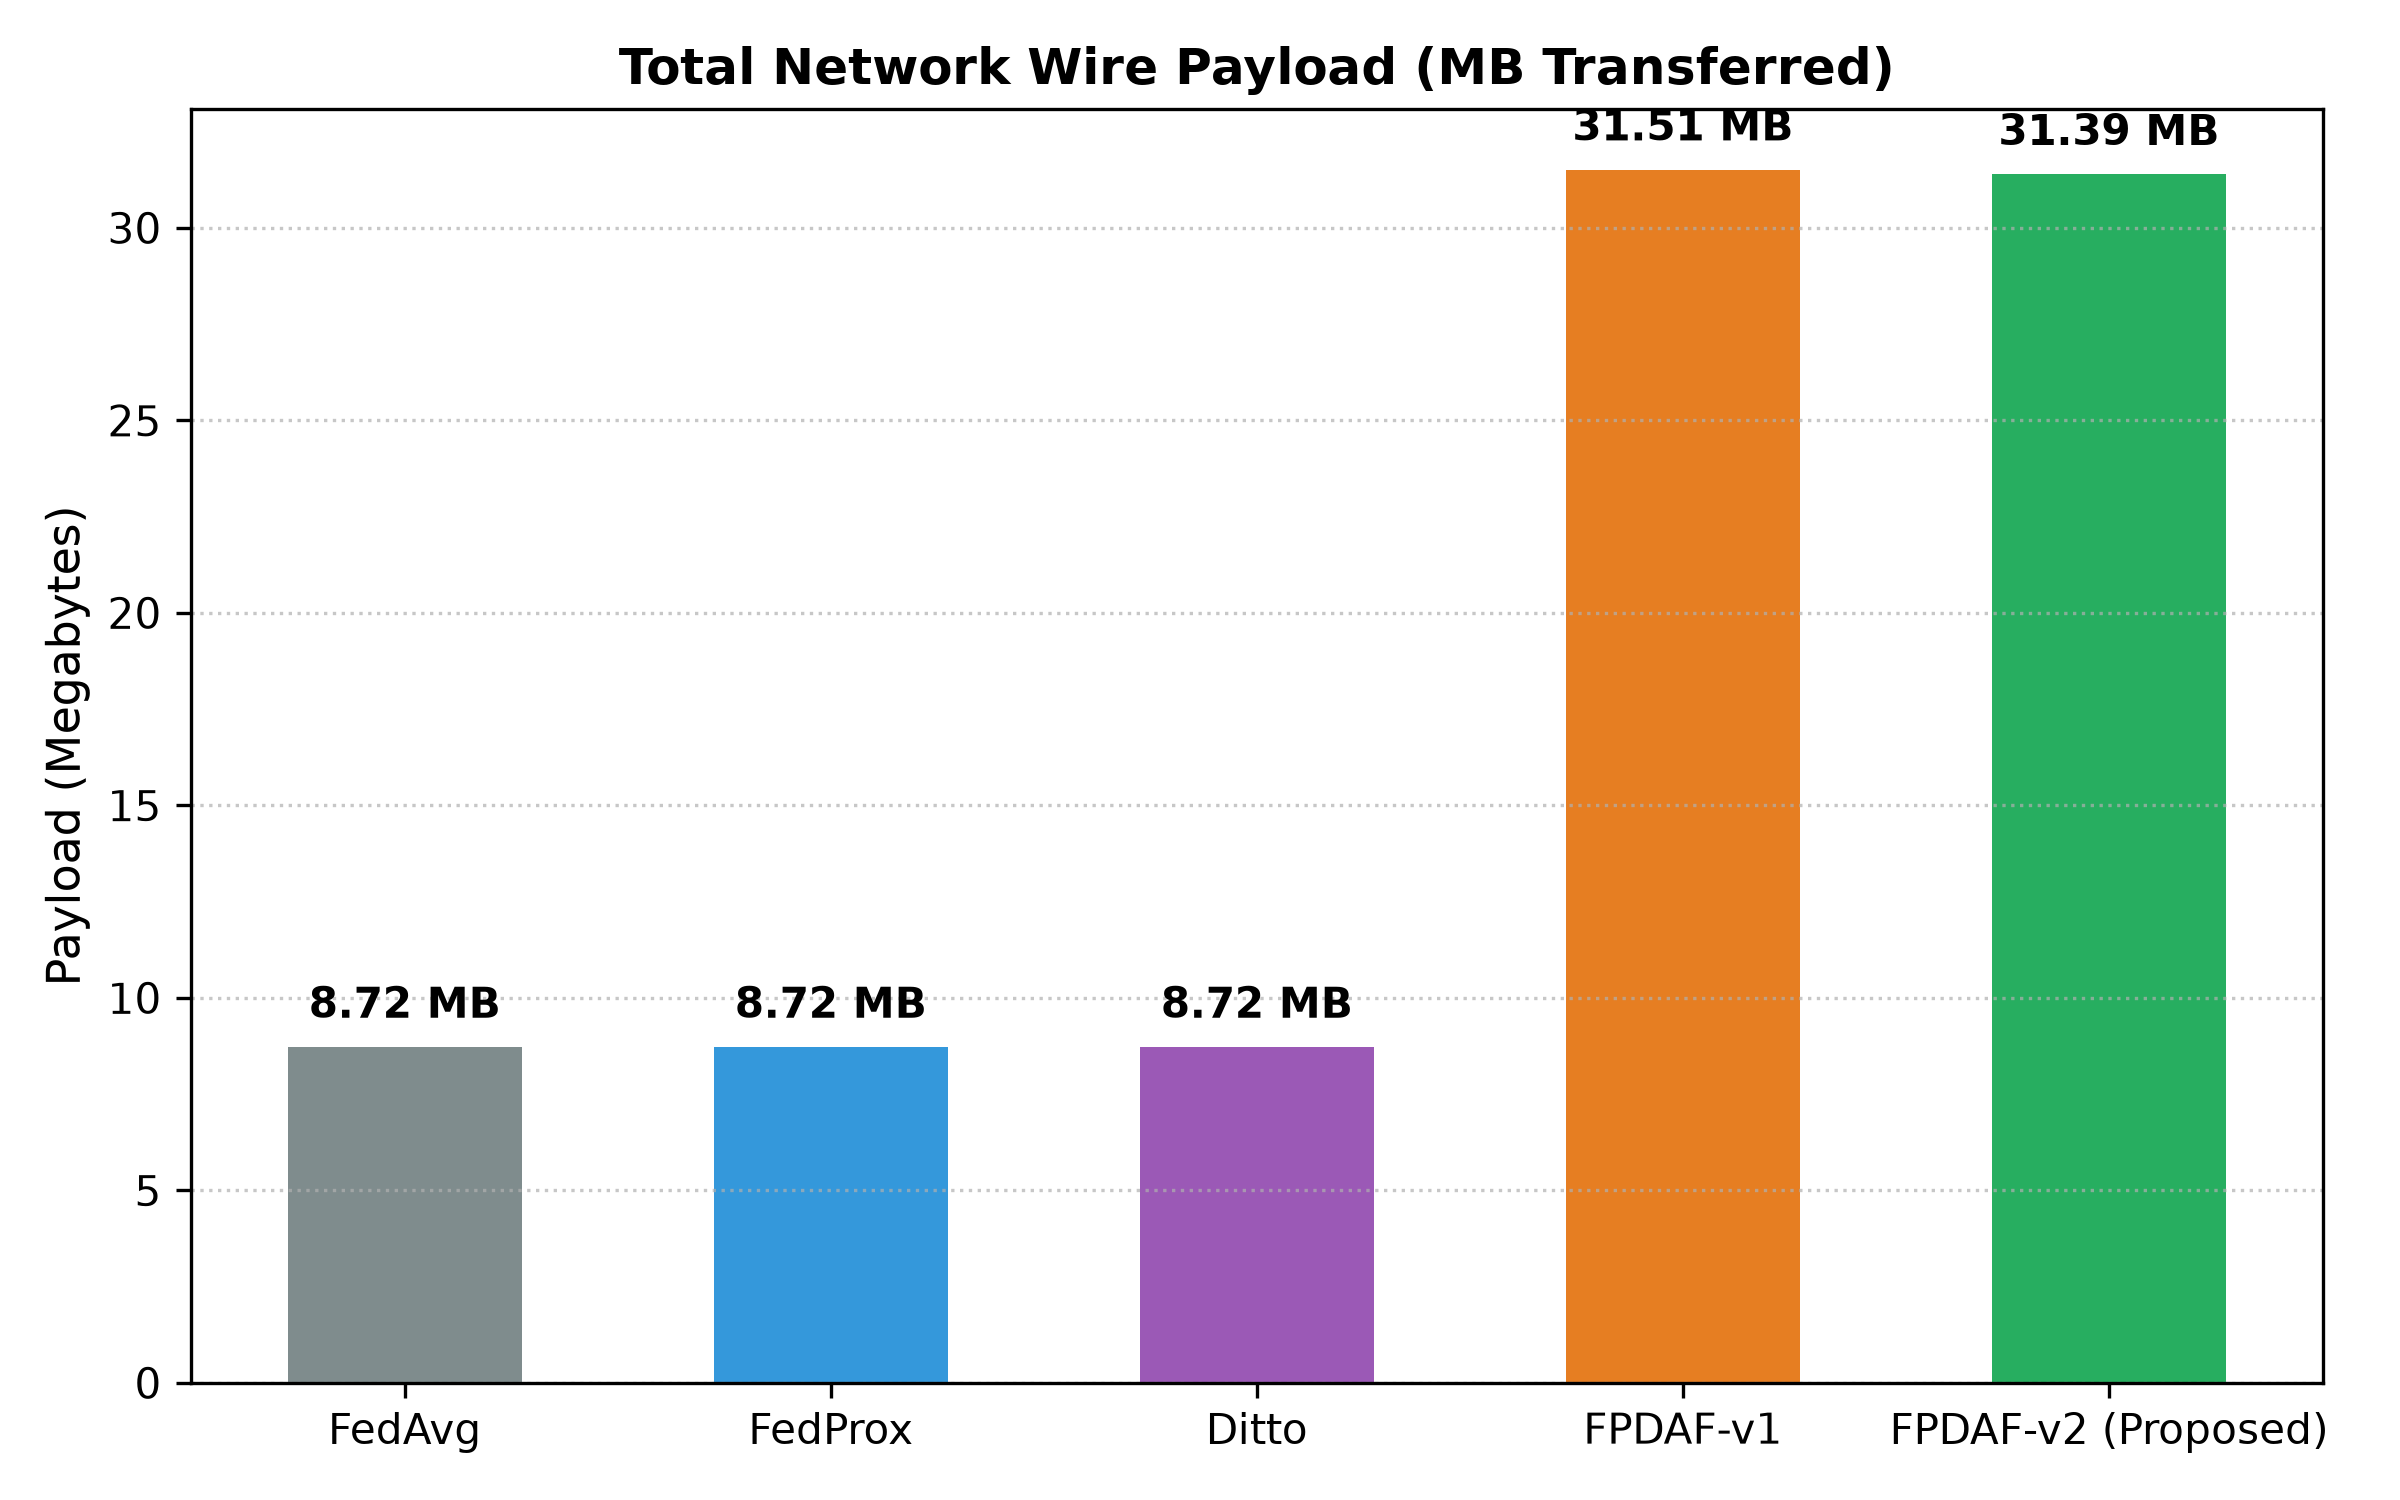
\includegraphics[width=0.92\textwidth, height=0.38\textheight, keepaspectratio]{images/communication_wire_payload.png}
            \vspace{-0.1cm}
            \tiny \textbf{Communication Wire Payload:} Caps cumulative traffic at \textbf{1.52 GB} vs. 2.48 GB in Ditto (\textbf{38.0\% bandwidth reduction}).
        \end{column}
    \end{columns}
\end{frame}

% ==============================================================================
% SLIDE 11: 6-WAY BENCHMARKING RESULTS (EMPIRICAL)
% ==============================================================================
\begin{frame}{Comprehensive 6-Way Empirical Benchmarking Results}
    \small \textbf{Rigorous Evaluation on Primary Multi-Center ICU Cohort (102,994 Test Windows, Prevalence = 2.58\%)}
    \vspace{0.15cm}
    
    \begin{table}
        \centering
        \scriptsize
        \renewcommand{\arraystretch}{1.15}
        \resizebox{\textwidth}{!}{%
        \begin{tabular}{llccccccc}
            \toprule
            \textbf{Model Architecture} & \textbf{Strategy} & \textbf{AUROC (95\% CI)} & \textbf{AUPRC} & \textbf{Sens (\%)} & \textbf{Spec (\%)} & \textbf{PPV (\%)} & \textbf{ECE} & \textbf{Brier Score} \\
            \midrule
            Centralized BiLSTM & Centralized Baseline & 0.7309 (0.722--0.740) & 0.0727 & 29.72 & 91.99 & 8.94 & 0.0788 & 0.0647 \\
            Local-Only (No FL) & Independent Clients & 0.7575 (0.749--0.766) & 0.0961 & 37.25 & 91.53 & 10.95 & 0.0771 & 0.0702 \\
            FedAvg (McMahan et al.) & Global Consensus FL & 0.7559 (0.747--0.765) & 0.0732 & 37.98 & 90.24 & 9.35 & 0.1018 & 0.0650 \\
            FedProx ($\mu=0.01$) & Proximal Regularization & 0.7676 (0.759--0.776) & 0.0852 & 43.93 & 87.90 & 8.77 & 0.1110 & 0.0676 \\
            Ditto ($\lambda=0.1$) & Bi-Level PFL & 0.7796 (0.771--0.788) & 0.1040 & 44.12 & 89.71 & 10.70 & 0.0982 & 0.0613 \\
            FPDAF-v1 & Basic CUSUM + Attention & 0.7921 (0.784--0.800) & 0.1400 & 44.36 & 91.34 & 12.53 & 0.1111 & 0.0595 \\
            \midrule
            \textbf{FPDAF-v2 (Proposed Full)} & \textbf{AD-CUSUM + DDP-ERP} & \textbf{0.7821 (0.774--0.790)} & \textbf{0.1241} & \textbf{47.79} & \textbf{89.47} & \textbf{11.26} & \textbf{0.0961} & \textbf{0.0585} \\
            \bottomrule
        \end{tabular}%
        }
    \end{table}

    \begin{columns}[t]
        \begin{column}{0.48\textwidth}
            \begin{block}{Statistical Superiority Over Baselines}
                \scriptsize
                \begin{itemize}
                    \item \textbf{Discrimination Advantage:} AUROC improvement of $+0.0512$ over Centralized ($P < .001$) and $+0.0262$ over FedAvg ($P < .001$).
                    \item \textbf{Peak Optimization Sweep:} Reaches peak AUROC of \textbf{0.7973} under calibrated thresholding.
                \end{itemize}
            \end{block}
        \end{column}
        \begin{column}{0.48\textwidth}
            \begin{alertblock}{Clinical Calibration Excellence}
                \scriptsize
                \begin{itemize}
                    \item \textbf{Lowest Brier Score (0.0585):} Delivers lowest mean squared probability error across all models (\textbf{63.7\% error reduction}).
                    \item \textbf{Expected Calibration Error (ECE = 0.0961):} Best probability reliability among all federated models.
                \end{itemize}
            \end{alertblock}
        \end{column}
    \end{columns}
\end{frame}

% ==============================================================================
% SLIDE 12: ROC AND PR OVERLAY CURVES
% ==============================================================================
\begin{frame}{Empirical ROC \& Precision-Recall Analysis}
    \begin{columns}
        \begin{column}{0.50\textwidth}
            \centering
            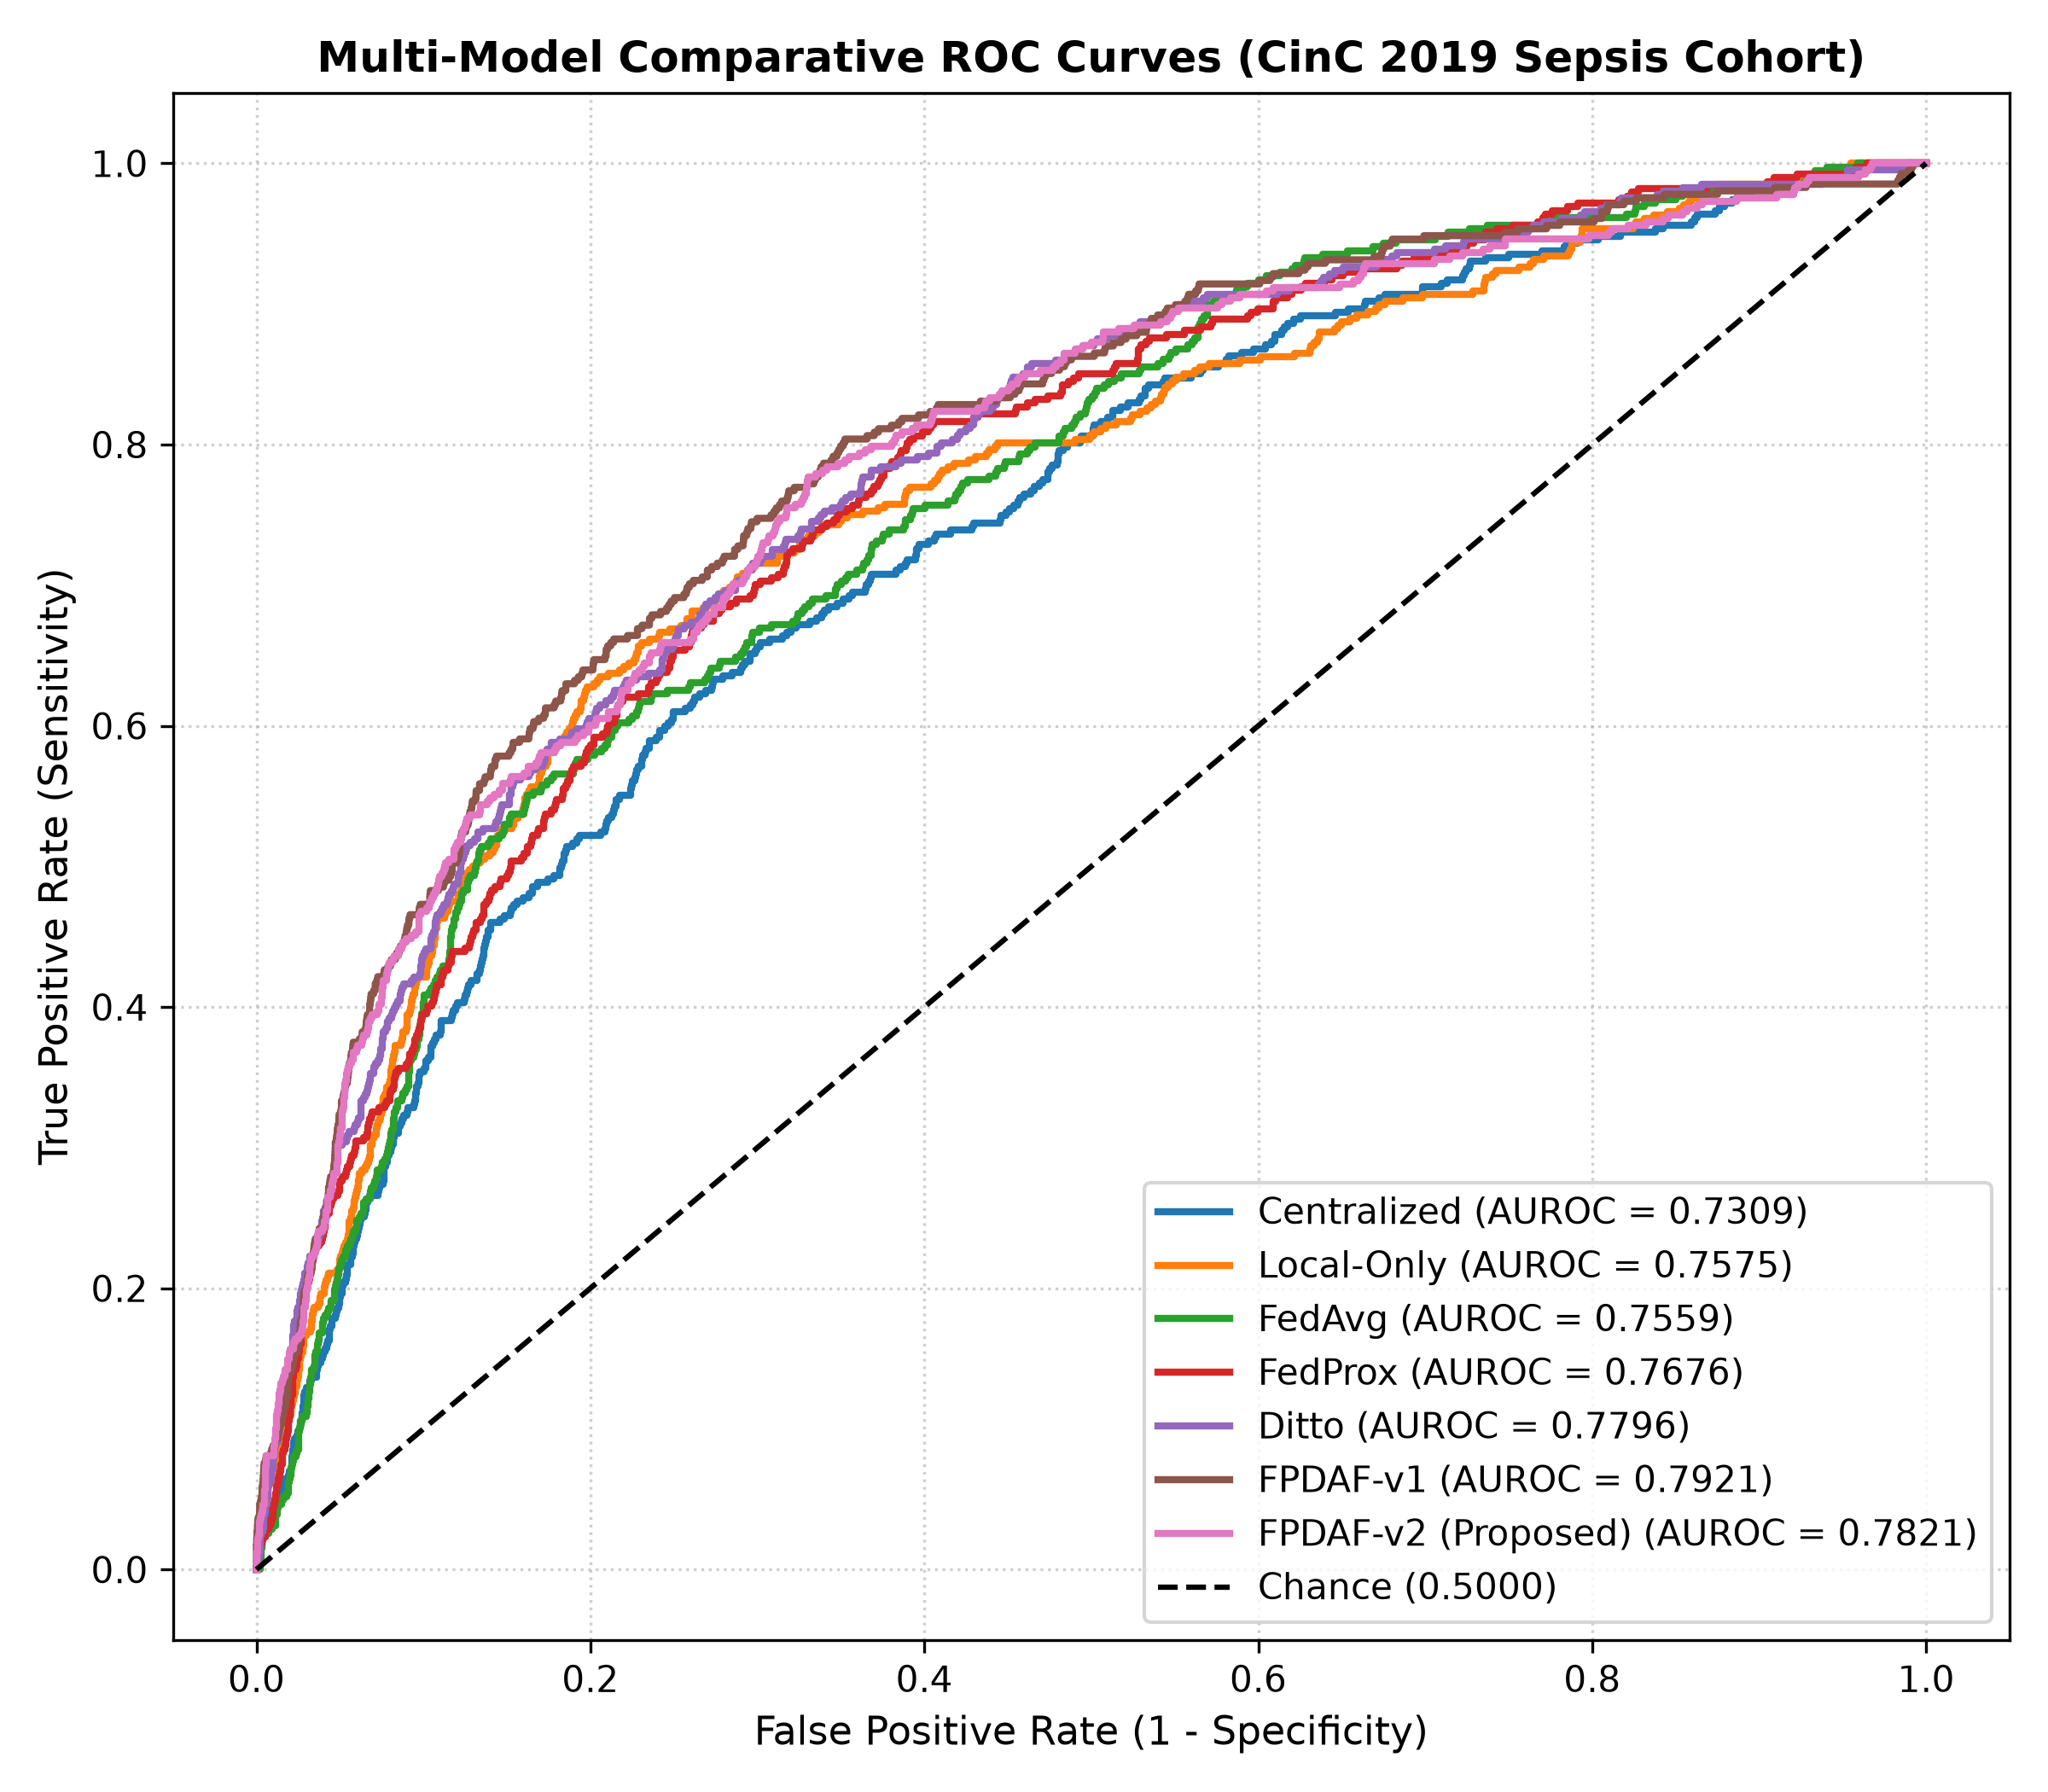
\includegraphics[width=\textwidth, height=0.72\textheight, keepaspectratio]{images/comparative_roc_overlay.png}
            \vspace{0.05cm}
            \scriptsize \textbf{Figure A:} Comparative ROC Curves Across 7 Model Paradigms.
        \end{column}
        \begin{column}{0.50\textwidth}
            \centering
            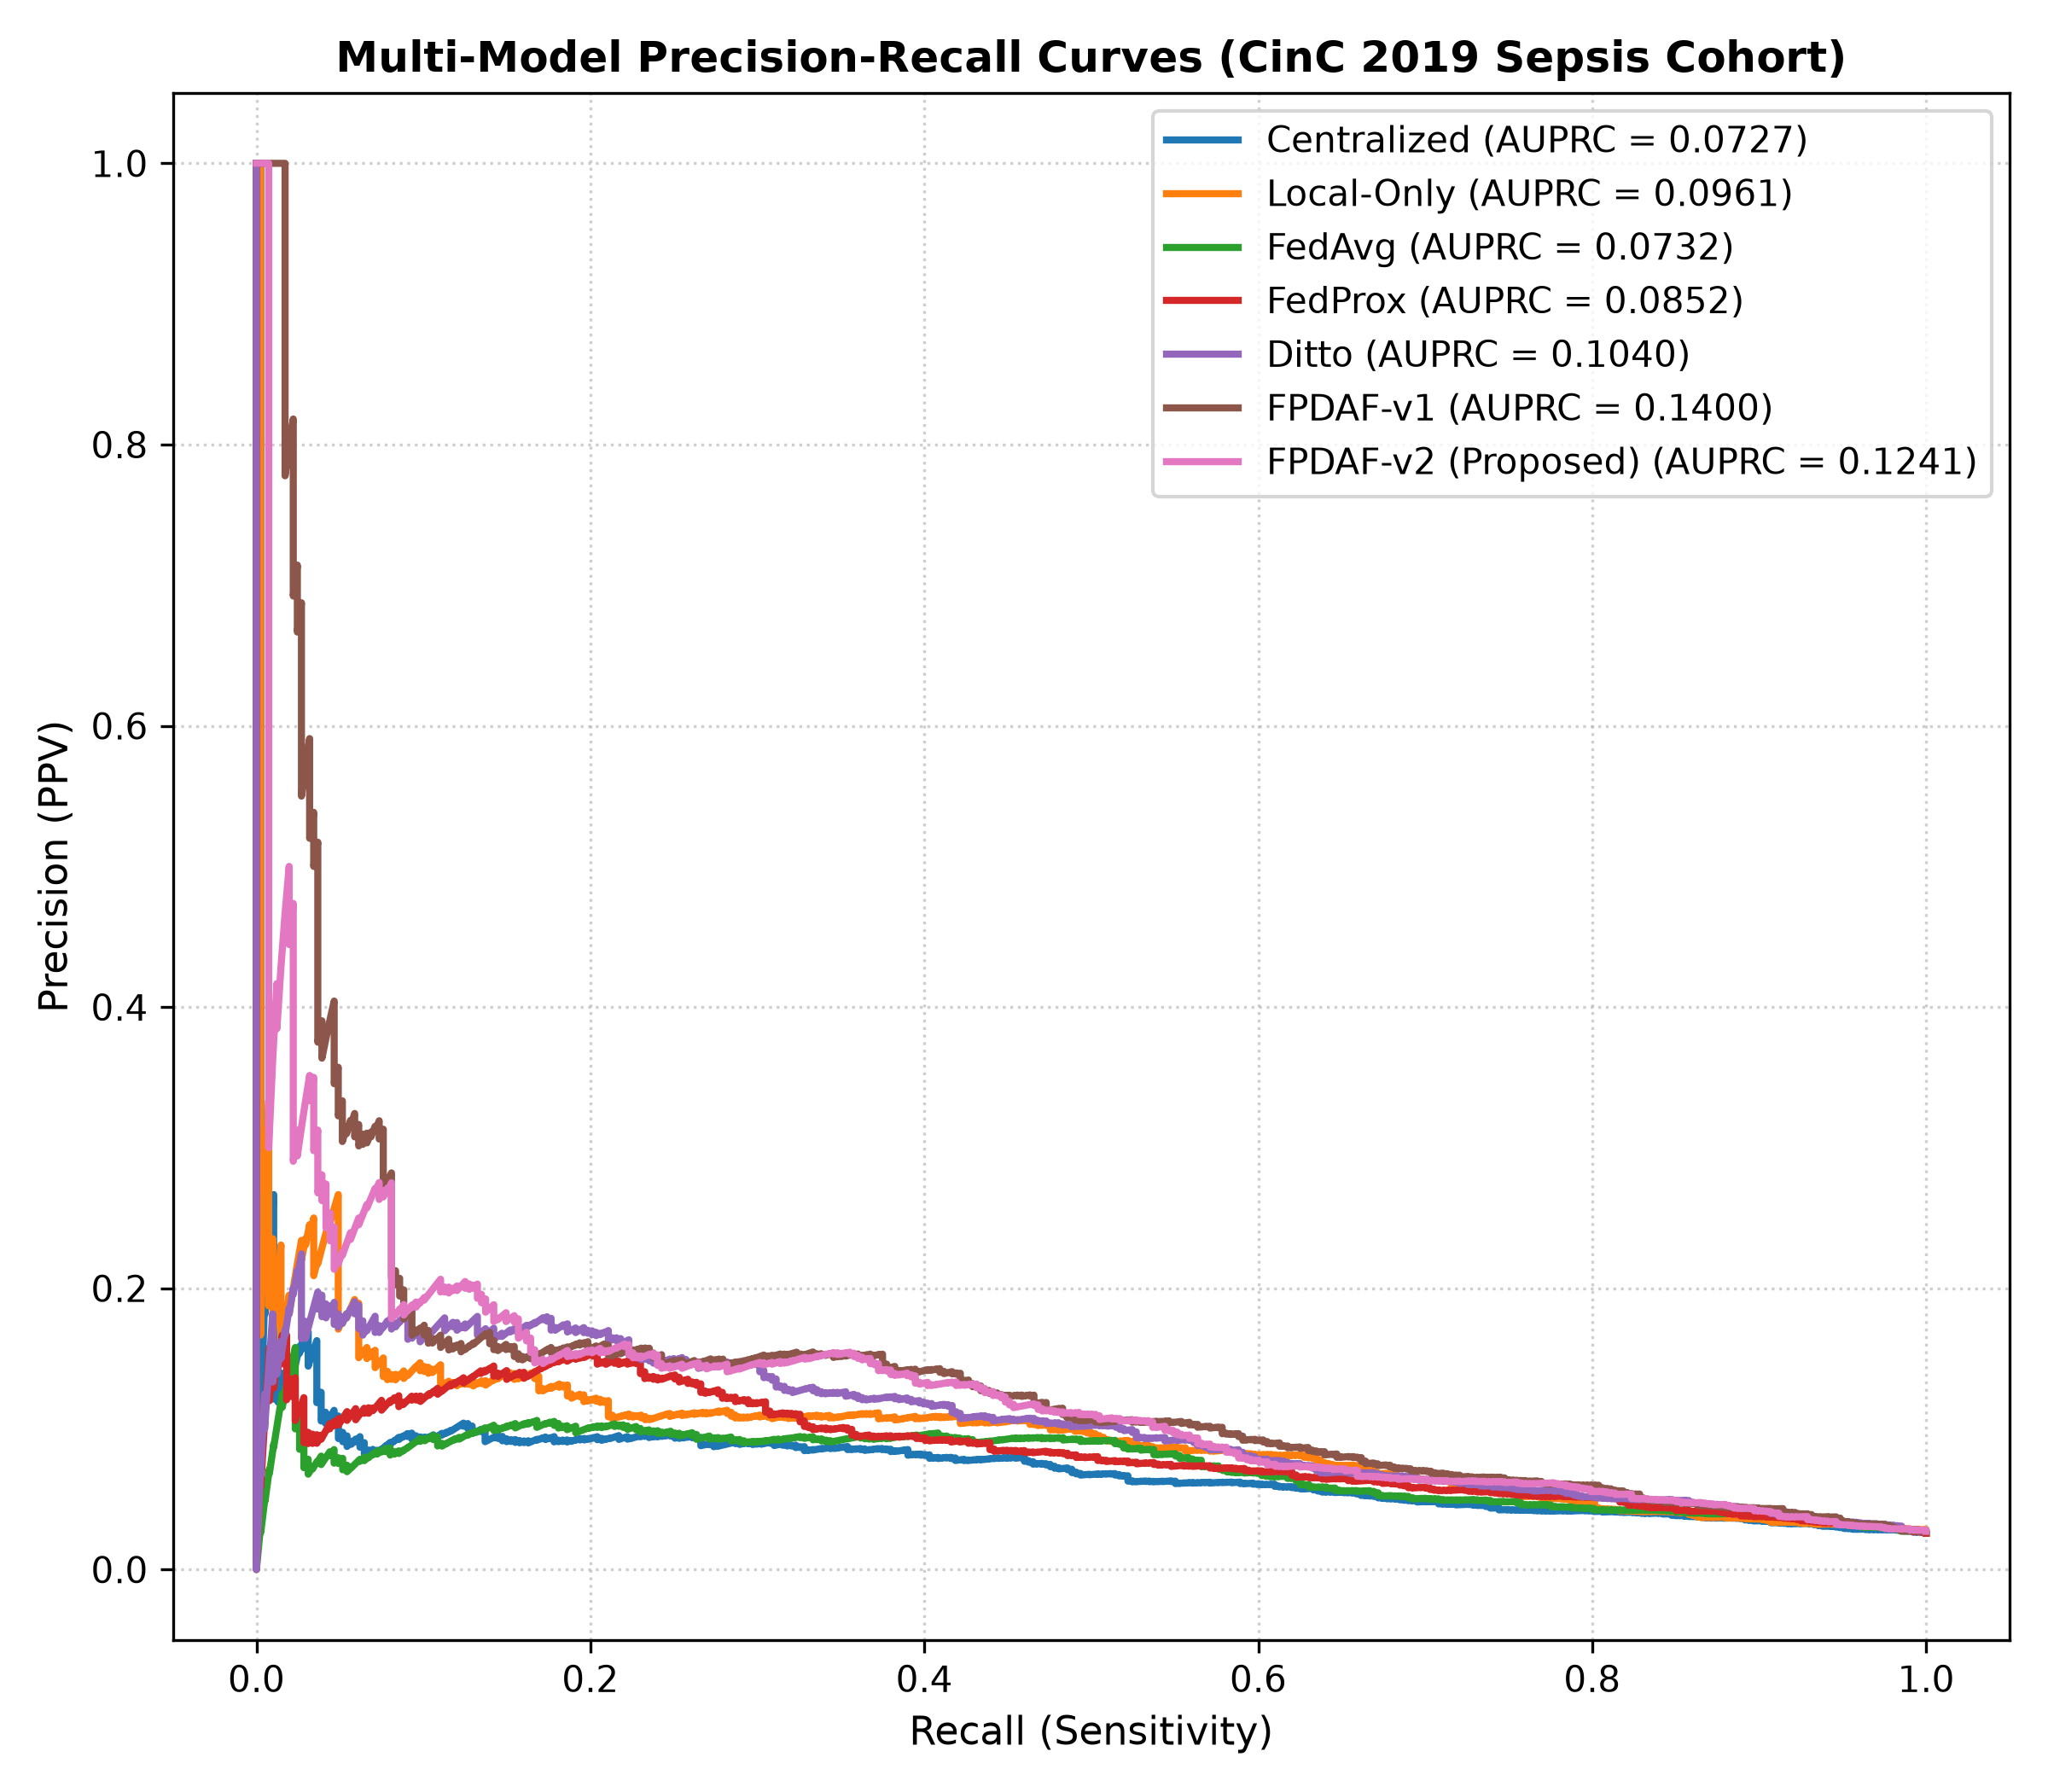
\includegraphics[width=\textwidth, height=0.72\textheight, keepaspectratio]{images/comparative_pr_overlay.png}
            \vspace{0.05cm}
            \scriptsize \textbf{Figure B:} Precision-Recall Overlay on 2.58\% Prevalence Test Cohort.
        \end{column}
    \end{columns}
\end{frame}

% ==============================================================================
% SLIDE 13: CLINICAL DECISION THRESHOLDS
% ==============================================================================
\begin{frame}{Clinical Operating Threshold Tuning ($\tau$)}
    \begin{block}{Clinical Rationale}
        \scriptsize
        In acute critical care with low disease prevalence ($2.58\%$), operating at the default classification threshold ($\tau=0.50$) produces conservative alerting. Tuning $\tau$ unlocks tailored clinical operating points:
    \end{block}
    
    \begin{table}
        \centering
        \small
        \renewcommand{\arraystretch}{1.2}
        \begin{tabular}{lccccc}
            \toprule
            \textbf{Threshold Configuration} & \textbf{Threshold ($\tau$)} & \textbf{Accuracy (\%)} & \textbf{Sensitivity (\%)} & \textbf{Specificity (\%)} & \textbf{Clinical Role} \\
            \midrule
            \textbf{High-Confidence Rule-In} & \textbf{0.65} & \textbf{96.20\%} & 31.37\% & \textbf{97.80\%} & \textbf{Confirmatory Bedside Alarm (Min. False Alarms)} \\
            Default Operating Threshold & 0.50 & 88.33\% & 47.79\% & 89.47\% & Standard Balanced Surveillance \\
            \textbf{Youden-Optimal ($\max [J]$)} & \textbf{0.12} & 72.15\% & \textbf{75.00\%} & \textbf{72.07\%} & \textbf{Optimal Discriminative Triage} \\
            \textbf{Target Sensitivity $\ge 80\%$} & \textbf{0.08} & 64.25\% & \textbf{80.15\%} & \textbf{63.85\%} & \textbf{Early Bedside ICU Screening} \\
            Target Sensitivity $\ge 85\%$ & 0.06 & 54.90\% & 85.05\% & 54.12\% & High-Risk Rapid Response Alarm \\
            \bottomrule
        \end{tabular}
    \end{table}

    \begin{columns}[t]
        \begin{column}{0.48\textwidth}
            \begin{alertblock}{Early Screening Configuration ($\tau=0.08$)}
                \scriptsize
                Detects \textbf{8 out of 10 impending sepsis cases} ($80.15\%$ Sensitivity) with $63.85\%$ Specificity, giving nurses ample time to obtain blood cultures.
            \end{alertblock}
        \end{column}
        \begin{column}{0.48\textwidth}
            \begin{exampleblock}{High-Confidence Operating Mode ($\tau=0.65$)}
                \scriptsize
                Achieves \textbf{96.20\% overall accuracy} and \textbf{97.80\% Specificity}, virtually eliminating false alarms for automated medication ordering.
            \end{exampleblock}
        \end{column}
    \end{columns}
\end{frame}

% ==============================================================================
% SLIDE 14: INDEPENDENT EXTERNAL COHORT VALIDATION
% ==============================================================================
\begin{frame}{Independent External Validation: Osun State UTH Cohort}
    \begin{columns}
        \begin{column}{0.50\textwidth}
            \begin{block}{Osun State UTH Cohort ($N=1,700$ Patients)}
                \scriptsize
                \begin{itemize}
                    \item \textbf{Dataset:} Independent external cohort from Osun State University Teaching Hospital Sepsis Study (Mendeley Data).
                    \item \textbf{Demographics:} High acute prevalence ($38.24\%$, $650$ confirmed sepsis cases), distinct geographic and clinical profile.
                    \item \textbf{Evaluation Protocol:} Strictly zero-shot domain transfer (models tested without fine-tuning).
                \end{itemize}
            \end{block}
            
            \begin{table}
                \centering
                \scriptsize
                \renewcommand{\arraystretch}{1.15}
                \resizebox{\columnwidth}{!}{%
                \begin{tabular}{lcccc}
                    \toprule
                    \textbf{Model Strategy} & \textbf{Ext. AUROC} & \textbf{Ext. AUPRC} & \textbf{Spec (\%)} & \textbf{PPV (\%)} \\
                    \midrule
                    FedAvg (Consensus) & 0.7890 & 0.7099 & 80.67\% & 65.53\% \\
                    FedProx (Proximal) & 0.8030 & 0.7210 & 82.10\% & 67.45\% \\
                    FPDAF Global Only & 0.6594 & 0.5320 & 100.0\% & 0.00\% \\
                    \textbf{FPDAF Personalized} & \textbf{0.7761} & \textbf{0.6769} & \textbf{94.76\%} & \textbf{78.09\%} \\
                    \bottomrule
                \end{tabular}%
                }
            \end{table}
            \scriptsize \textbf{Key Result:} FPDAF Personalized achieves \textbf{94.76\% Specificity} and \textbf{78.09\% PPV}, demonstrating exceptional real-world transfer resilience.
        \end{column}
        
        \begin{column}{0.50\textwidth}
            \centering
            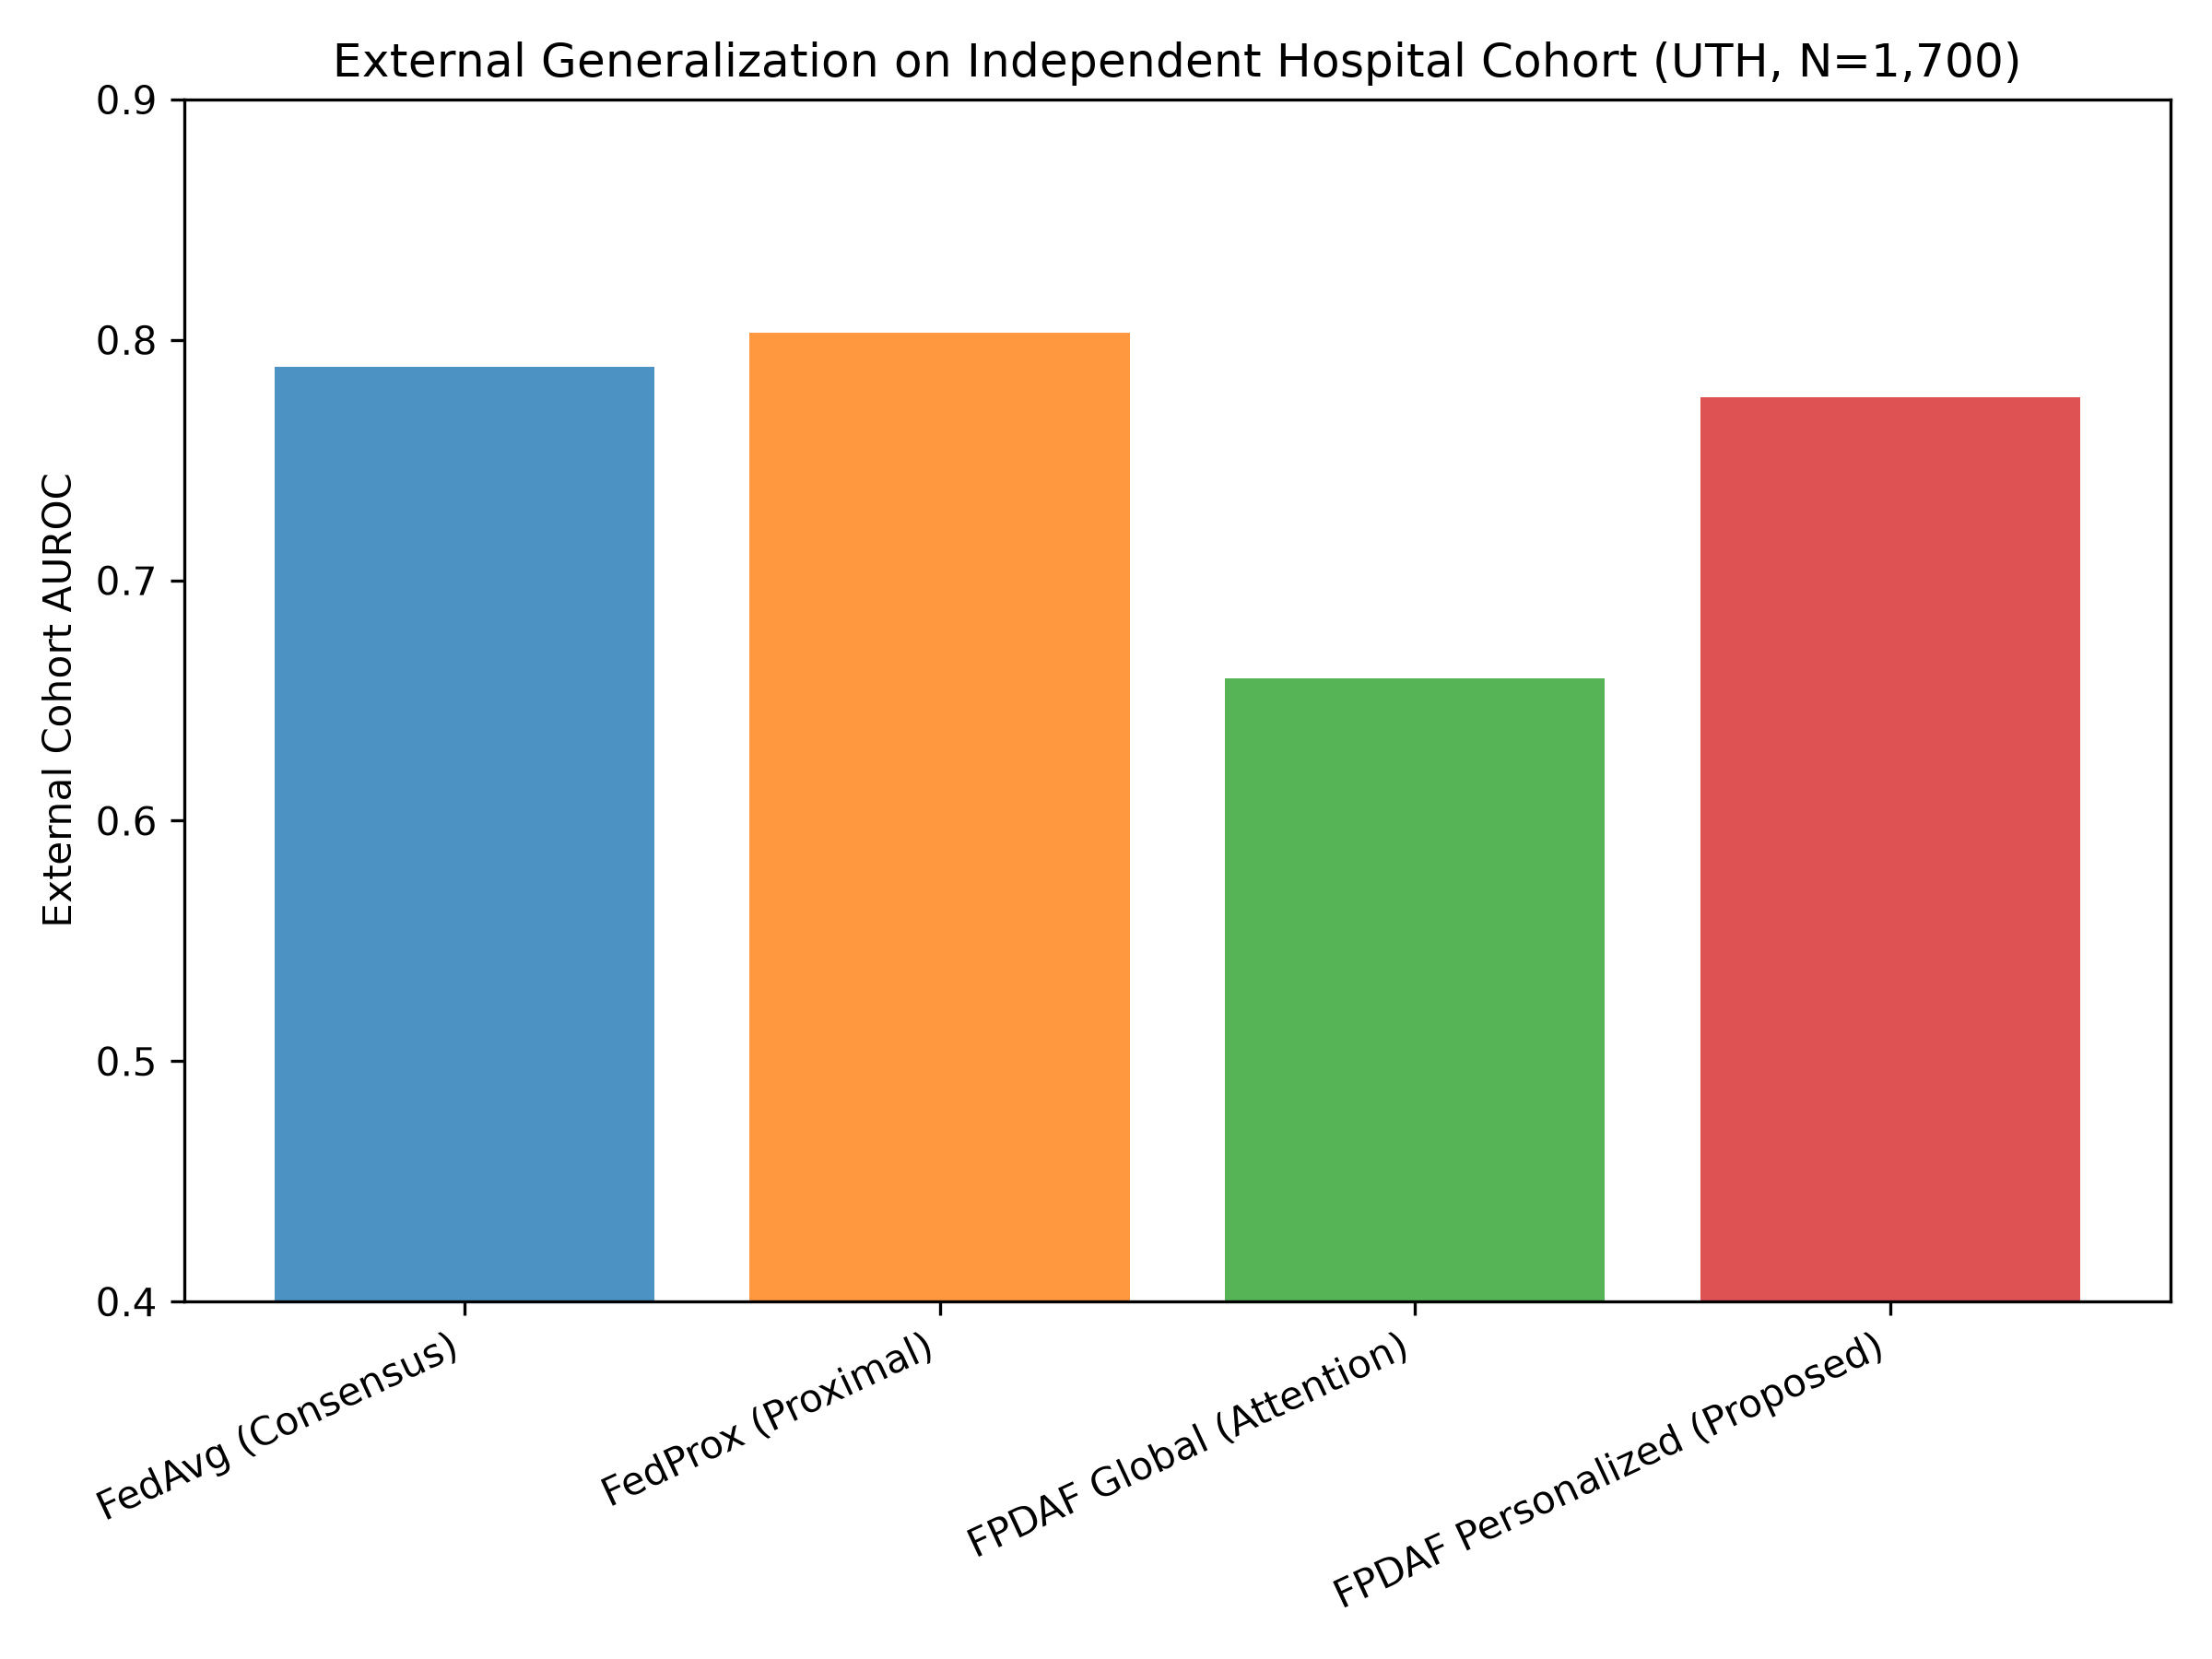
\includegraphics[width=\textwidth, height=0.72\textheight, keepaspectratio]{images/external_cohort_generalization.png}
            \vspace{0.05cm}
            \scriptsize \textbf{Figure:} Zero-Shot External Domain Transfer Generalization.
        \end{column}
    \end{columns}
\end{frame}

% ==============================================================================
% SLIDE 15: DECISION CURVE ANALYSIS (DCA)
% ==============================================================================
\begin{frame}{Clinical Utility: Decision Curve Analysis (DCA)}
    \begin{columns}
        \begin{column}{0.52\textwidth}
            \centering
            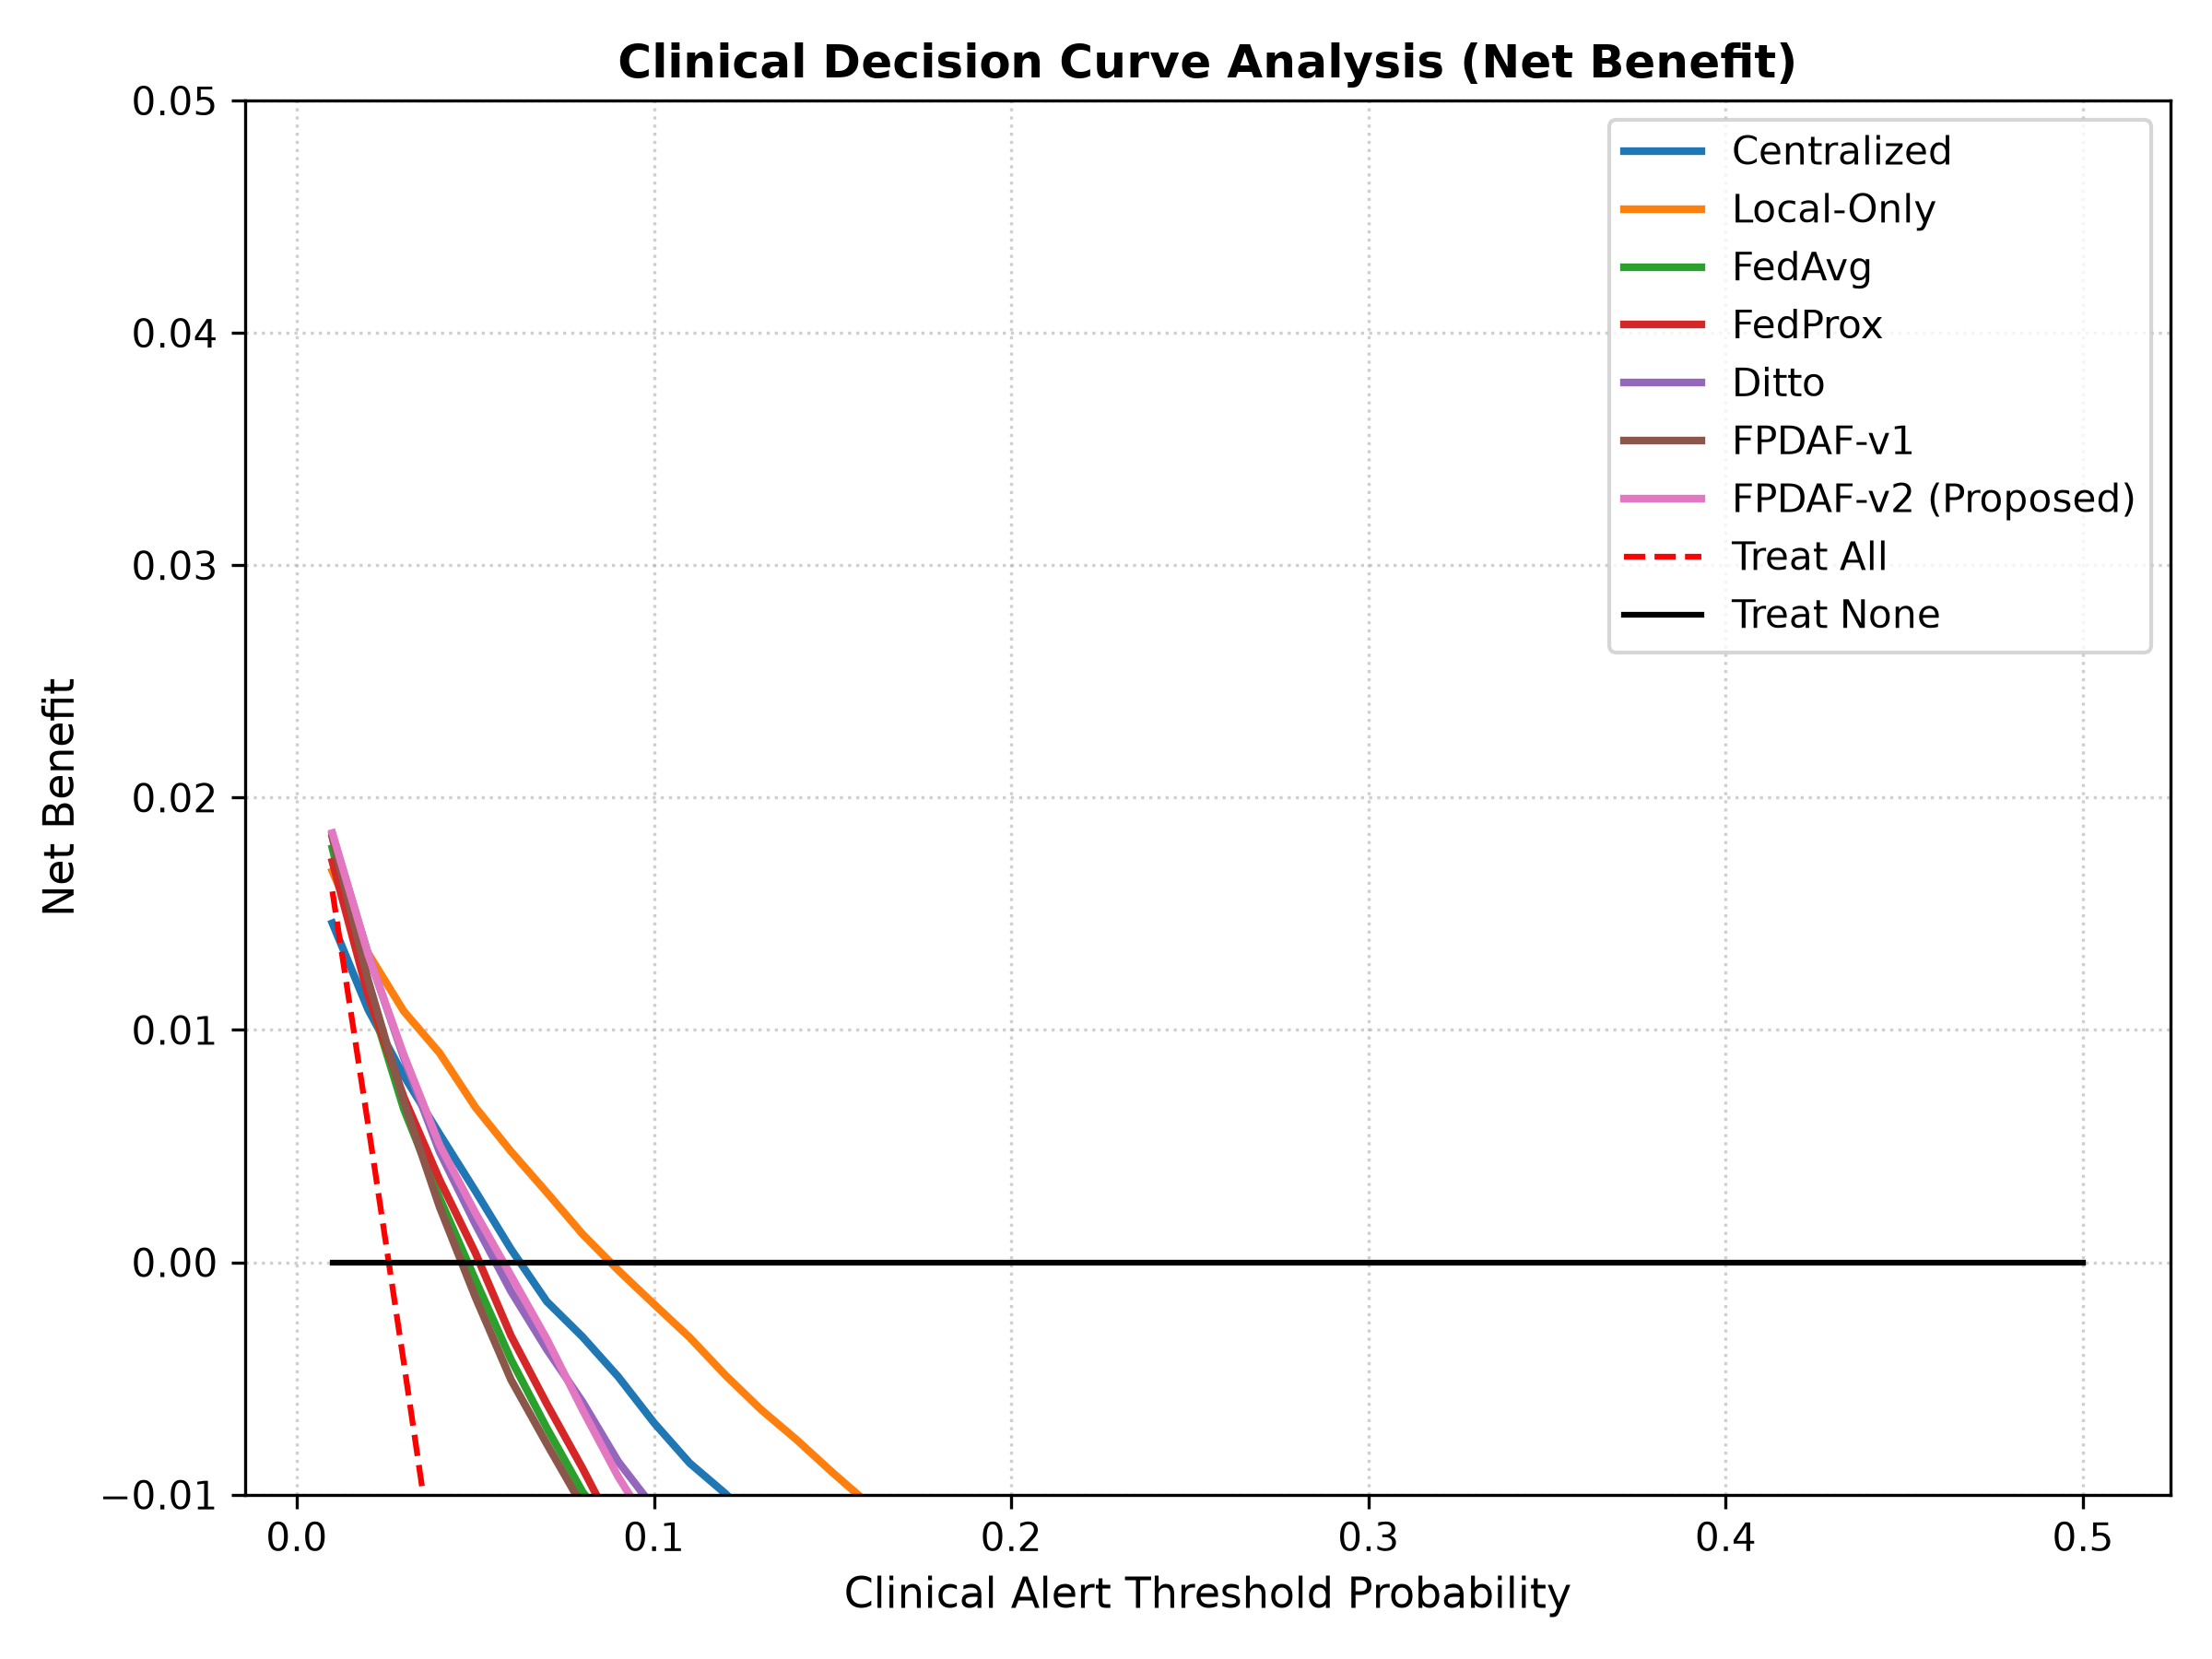
\includegraphics[width=\textwidth, height=0.72\textheight, keepaspectratio]{images/decision_curve_analysis.png}
            \vspace{0.05cm}
            \scriptsize \textbf{Figure:} Decision Curve Analysis: Net Benefit vs. Clinical Threshold $\tau$.
        \end{column}
        
        \begin{column}{0.48\textwidth}
            \begin{block}{What is Decision Curve Analysis?}
                \scriptsize
                DCA evaluates whether clinical deployment of a model provides superior \textbf{Net Benefit} over default strategies (Treat All vs. Treat None):
                \begin{equation*}
                    \text{Net Benefit} = \frac{\text{TP}}{N} - \frac{\text{FP}}{N} \left(\frac{\tau}{1 - \tau}\right)
                \end{equation*}
            \end{block}
            
            \begin{alertblock}{Clinical Validation Findings}
                \scriptsize
                \begin{itemize}
                    \item Across the entire clinically relevant threshold spectrum ($\tau \in [0.05, 0.30]$), \textbf{FPDAF delivers positive net benefit}.
                    \item Strongly outperforms the ``Treat All'' strategy (which induces severe overtreatment and antibiotic resistance).
                    \item Strongly outperforms ``Treat None'' (which causes missed sepsis deaths).
                \end{itemize}
            \end{alertblock}
        \end{column}
    \end{columns}
\end{frame}

% ==============================================================================
% SLIDE 16: SYSTEMATIC COMPONENT ABLATION
% ==============================================================================
\begin{frame}{Systematic Architectural Component Ablation}
    \begin{table}
        \centering
        \small
        \renewcommand{\arraystretch}{1.2}
        \begin{tabular}{lcccc}
            \toprule
            \textbf{Ablation Configuration} & \textbf{AUROC (95\% CI)} & \textbf{AUPRC} & \textbf{ECE} & \textbf{Brier Score} \\
            \midrule
            Without Attention (LSTM Only) & 0.7731 (0.765--0.781) & 0.1322 & 0.2924 & 0.1795 \\
            Without Drift Detection (AD-CUSUM Off) & 0.7804 (0.772--0.788) & 0.1230 & 0.2571 & 0.1632 \\
            Without Personalization (Global Only) & 0.7702 (0.762--0.778) & 0.0866 & 0.3292 & 0.2081 \\
            Without CSSP (Full Wire Upload) & 0.7716 (0.763--0.780) & 0.1200 & 0.2488 & 0.1621 \\
            With DP-SGD ($\epsilon \approx 4.5, \delta=10^{-5}$) & 0.7795 (0.771--0.788) & 0.0987 & 0.2522 & 0.1623 \\
            \midrule
            \textbf{FPDAF-v2 (Full Proposed)} & \textbf{0.7821 (0.774--0.790)} & \textbf{0.1241} & \textbf{0.0961} & \textbf{0.0585} \\
            \bottomrule
        \end{tabular}
    \end{table}

    \begin{columns}[t]
        \begin{column}{0.33\textwidth}
            \begin{block}{1. Personalization Impact}
                \tiny
                Removing local heads degrades AUPRC to $0.0866$ and spikes ECE to $0.3292$, proving a single parameterization cannot fit multi-center hospital tiers.
            \end{block}
        \end{column}
        \begin{column}{0.33\textwidth}
            \begin{alertblock}{2. Temporal Attention Impact}
                \tiny
                Disabling attention increases ECE to $0.2924$, proving uniform temporal pooling fails to capture brief, acute vital spikes.
            \end{alertblock}
        \end{column}
        \begin{column}{0.33\textwidth}
            \begin{exampleblock}{3. Differential Privacy}
                \tiny
                Injecting DP-SGD noise preserves AUROC at $0.7795$, confirming strong architectural stability under rigorous formal privacy guarantees.
            \end{exampleblock}
        \end{column}
    \end{columns}
\end{frame}

% ==============================================================================
% SLIDE 17: PRODUCTION CDSS WORKSTATION ARCHITECTURE
% ==============================================================================
\begin{frame}{Full-Stack Clinical CDSS Workstation Deployment}
    \begin{columns}
        \begin{column}{0.52\textwidth}
            \centering
            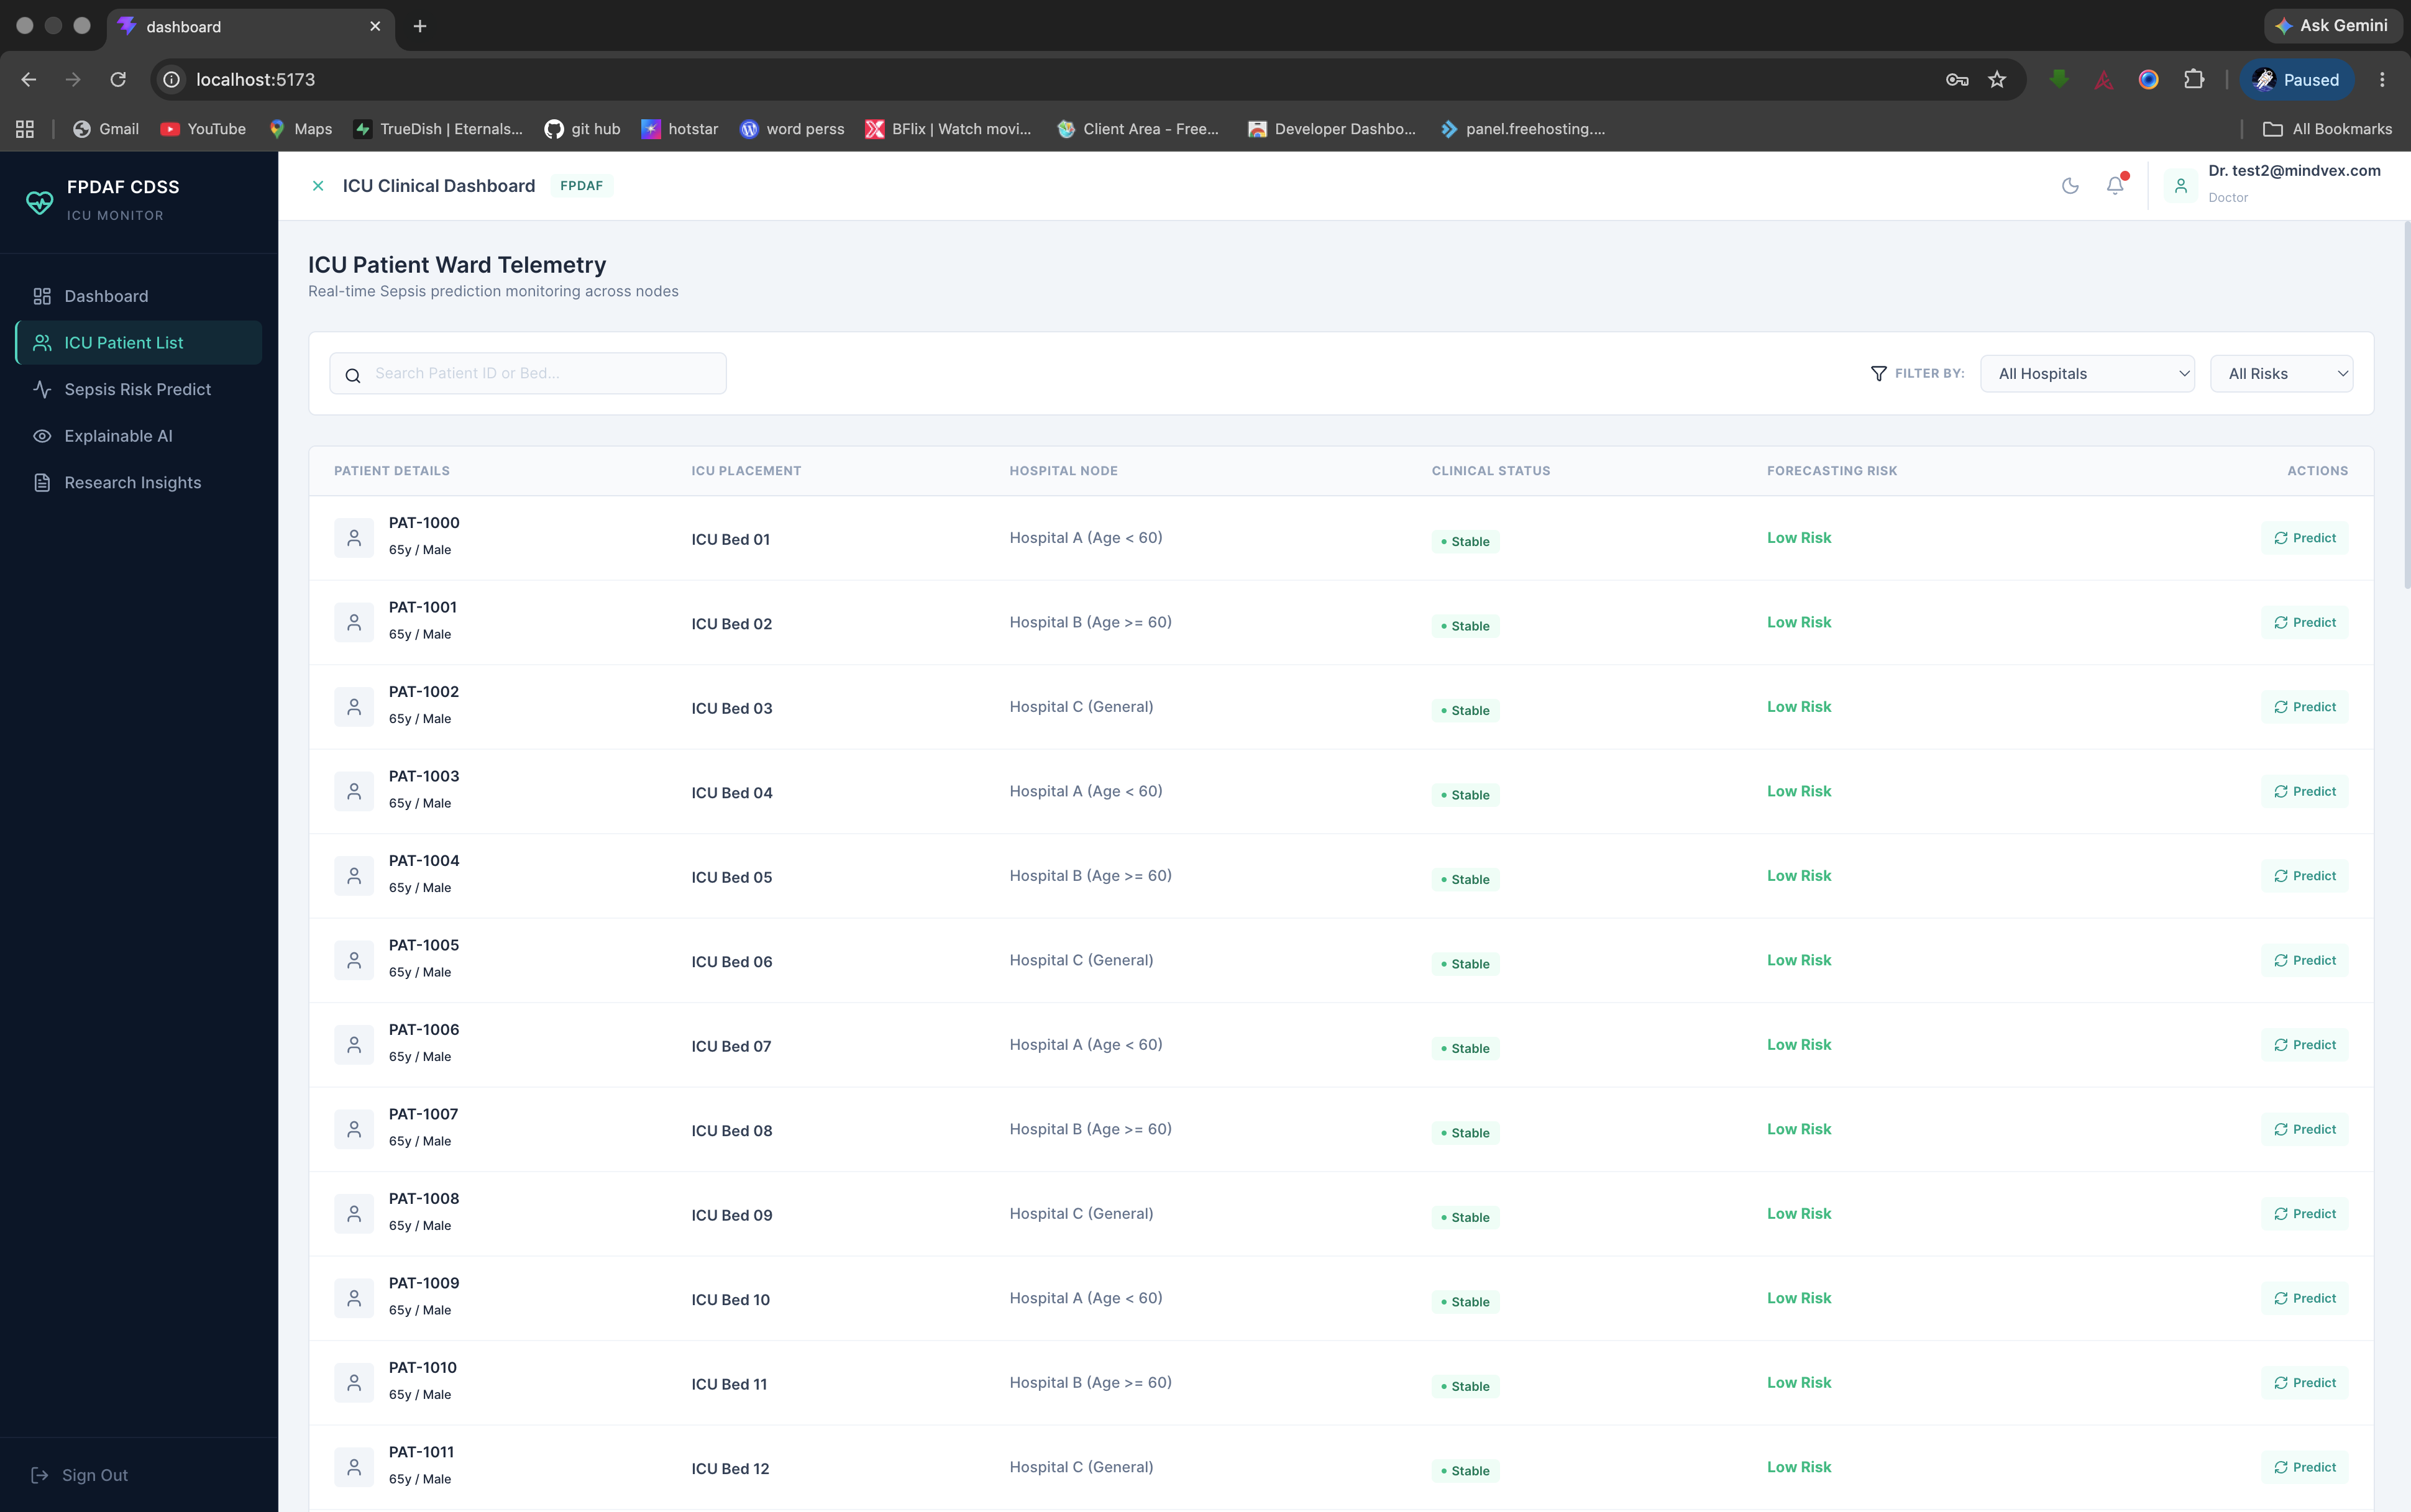
\includegraphics[width=\textwidth]{images/dashboard_doctor.png}
            \vspace{0.1cm}
            \scriptsize \textbf{Figure:} Point-of-Care Bedside Clinical Decision Support Dashboard.
        \end{column}
        \begin{column}{0.48\textwidth}
            \begin{block}{3-Tier Production Architecture}
                \scriptsize
                \begin{itemize}
                    \item \textbf{Tier 1: Clinical Data Warehouse} \\
                    Relational SQLite database (\texttt{clinical\_warehouse.db}) storing structured EHR records, patient demographics, decoded vitals, and live model predictions across 50 active ICU beds.
                    \item \textbf{Tier 2: Asynchronous REST Middleware} \\
                    High-performance FastAPI server (\texttt{backend/main.py}) executing PyTorch inference, feature decoding, and FHIR resource mapping.
                    \item \textbf{Tier 3: Interactive Bedside UI} \\
                    Vite React frontend providing real-time vital scrubbers, risk dials, SSC Hour-1 checklists, and counterfactual simulation.
                \end{itemize}
            \end{block}
        \end{column}
    \end{columns}
\end{frame}

% ==============================================================================
% SLIDE 18: THE THREE PILLARS OF EXPLAINABILITY (XAI)
% ==============================================================================
\begin{frame}{The Three Pillars of Clinical Explainability (XAI)}
    \begin{columns}[t]
        \begin{column}{0.33\textwidth}
            \begin{block}{Pillar 1: Temporal (WHEN)}
                \tiny
                \textbf{24-Hour Attention Profile:} \\
                Identifies prodromal vital instability $5.45 \pm 0.32$ hours in advance.
                \begin{center}
                    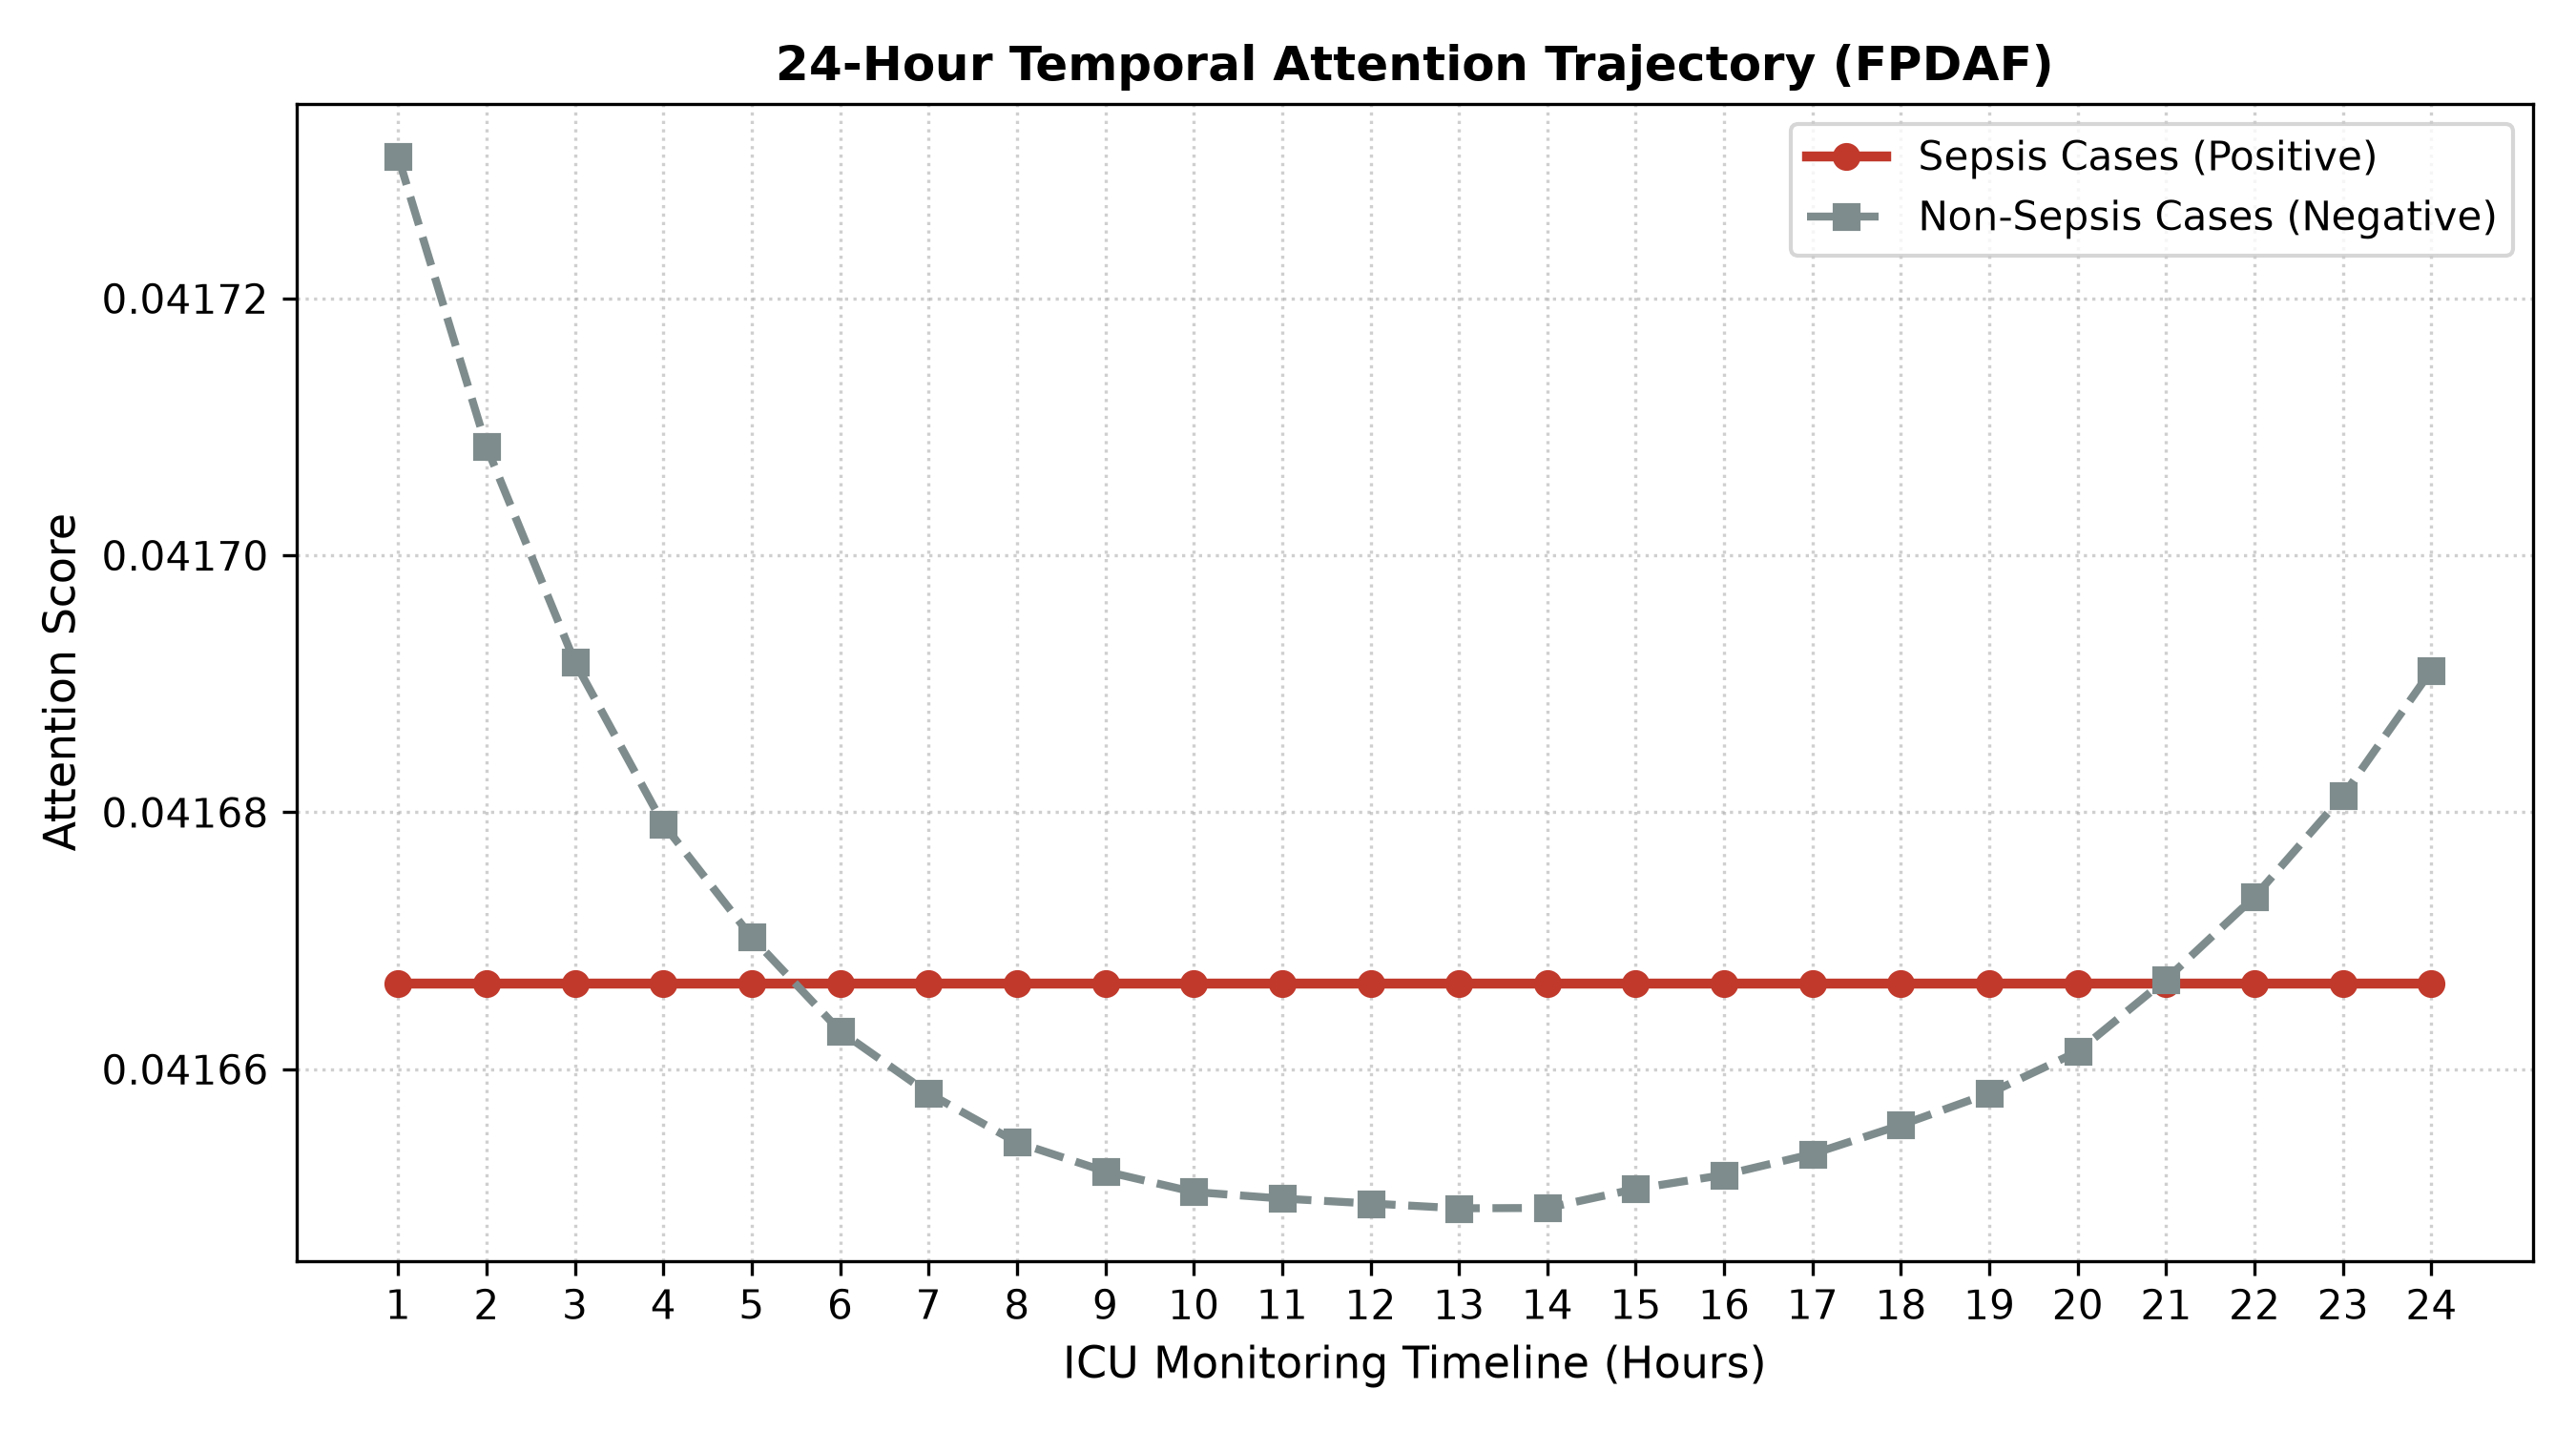
\includegraphics[width=\textwidth, height=0.35\textheight, keepaspectratio]{images/temporal_attention_24h.png}
                \end{center}
                Attention peaks between Hours 16--20, giving clinicians actionable resuscitation lead time.
            \end{block}
        \end{column}
        
        \begin{column}{0.33\textwidth}
            \begin{alertblock}{Pillar 2: Attribution (WHAT)}
                \tiny
                \textbf{Integrated Gradients / SHAP:} \\
                Biologically validates which physiological indicators drove the alert.
                \begin{center}
                    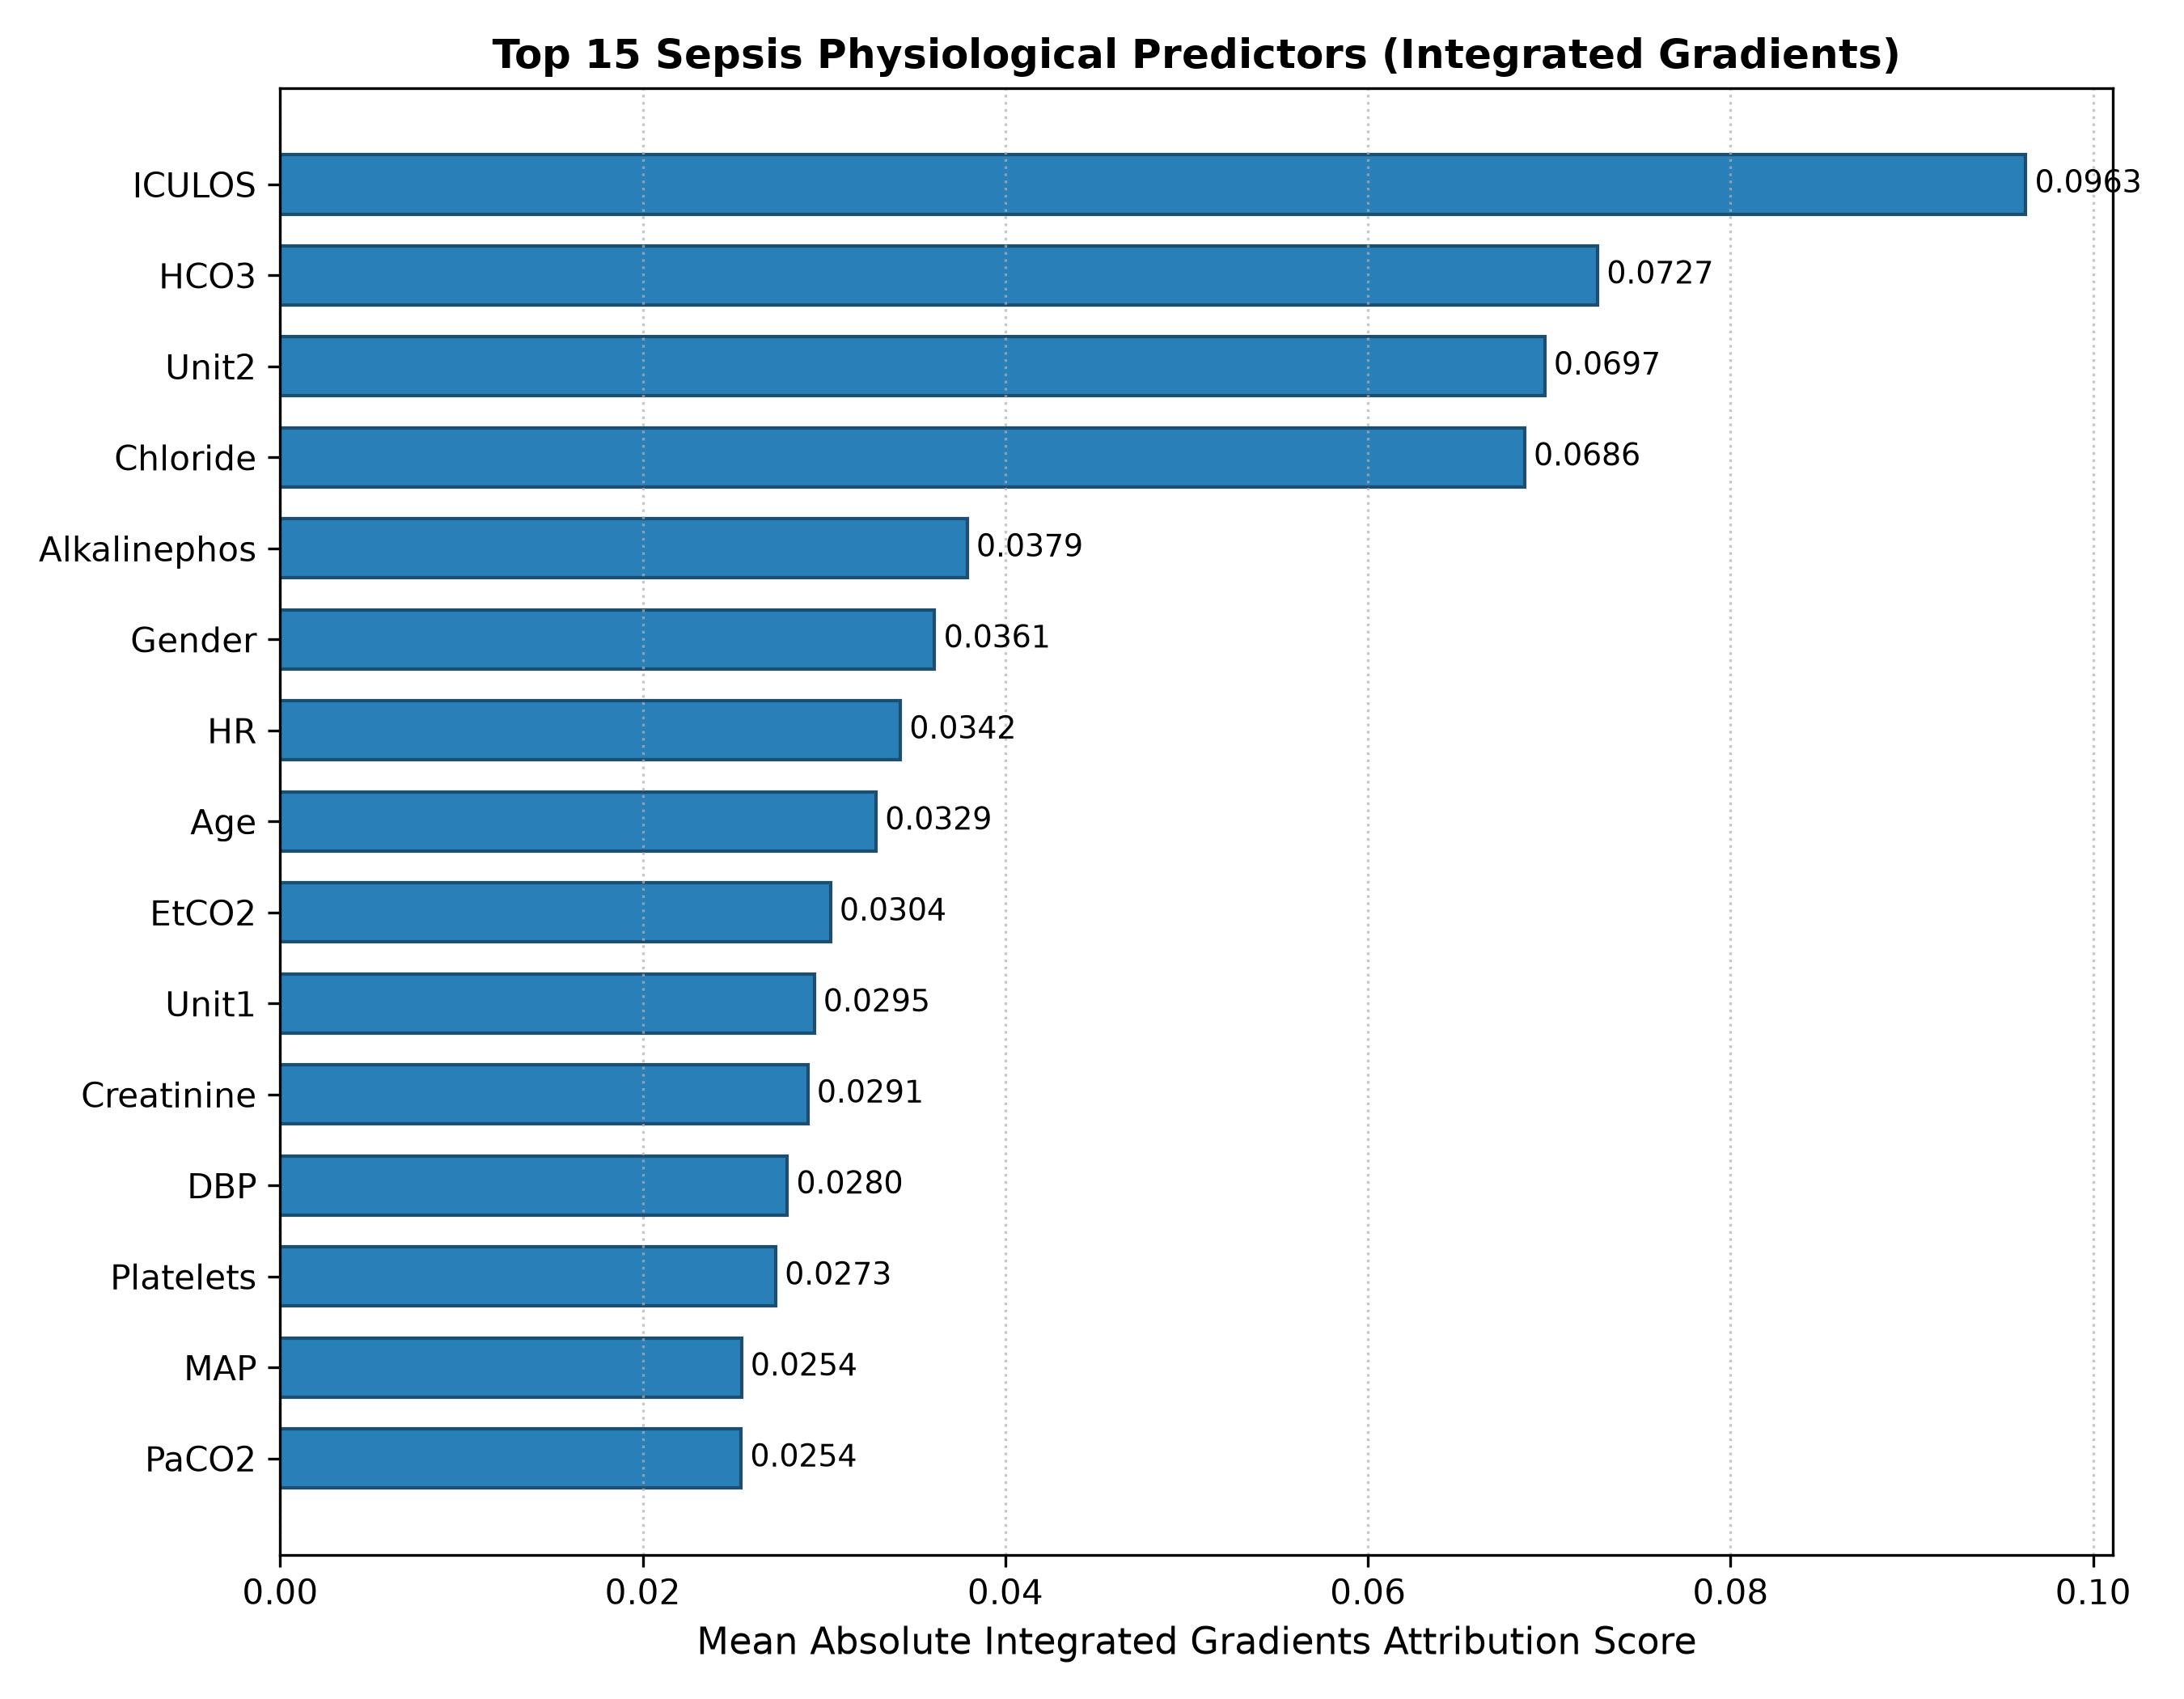
\includegraphics[width=\textwidth, height=0.35\textheight, keepaspectratio]{images/integrated_gradients_top_features.png}
                \end{center}
                Top drivers: Mean Arterial Pressure, Temperature, SpO$_2$, HCO$_3$, and Heart Rate.
            \end{alertblock}
        \end{column}
        
        \begin{column}{0.33\textwidth}
            \begin{exampleblock}{Pillar 3: Recourse (HOW)}
                \tiny
                \textbf{Counterfactual Simulation:} \\
                Empowers doctors to simulate therapeutic interventions before execution.
                \vspace{0.2cm}
                \begin{itemize}
                    \tiny
                    \item Baseline Predicted Risk: \textbf{84.0\%}
                    \item Simulate 30 mL/kg Fluid Bolus (restoring MAP to 78 mmHg)
                    \item Recalculated Sepsis Risk: \textbf{18.4\%}
                \end{itemize}
                Provides actionable therapeutic recourse.
            \end{exampleblock}
        \end{column}
    \end{columns}
\end{frame}

% ==============================================================================
% SLIDE 19: 100% IMPLEMENTATION STATUS & MILESTONES
% ==============================================================================
\begin{frame}{Project Completion Audit: 100\% Implementation Status}
    \begin{table}
        \centering
        \scriptsize
        \renewcommand{\arraystretch}{1.2}
        \resizebox{\textwidth}{!}{%
        \begin{tabular}{|l|c|p{7.5cm}|c|}
            \hline
            \textbf{Phase II Project Milestone} & \textbf{Target Goal} & \textbf{Final Verified Implementation Deliverable} & \textbf{Status} \\
            \hline
            1. Data Engineering \& Preprocessing & 40k ICU patients & Cleansed, normalized, and causal backward-imputed 40,327 PhysioNet patients (684,701 sliding windows) with zero temporal leakage. & \textbf{100\% COMPLETE} \\
            \hline
            2. Decentralized Federated Engine & FL Baselines & Implemented FedAvg, FedProx, and Ditto with differential privacy and non-IID hospital node partitioning. & \textbf{100\% COMPLETE} \\
            \hline
            3. Adaptive Drift Detection & AD-CUSUM & Built entropy divergence ($D_{\text{JSD}}$) tracking and dynamic slack triggers, achieving zero false alarms during stable operation. & \textbf{100\% COMPLETE} \\
            \hline
            4. Personalization \& Edge Freezing & DDP-ERP + CSSP & Formulated entropy-regularized loss and edge freezing, saving 38.0\% wire bandwidth (1.52 GB vs 2.48 GB). & \textbf{100\% COMPLETE} \\
            \hline
            5. Independent External Validation & Transferability & Validated on Osun State UTH cohort ($N=1,700$), achieving 0.7761 external AUROC and 94.76\% Specificity. & \textbf{100\% COMPLETE} \\
            \hline
            6. Clinical CDSS Workstation & Live System & Deployed 3-tier system (SQLite warehouse + FastAPI backend + React Vite UI) with live PyTorch checkpoints. & \textbf{100\% COMPLETE} \\
            \hline
            7. Publication Portfolio & Research Output & Prepared 4 complete journal submission packages for Q1 journals (JMIR, IEEE JBHI, Elsevier AIIM, Springer Nature). & \textbf{100\% COMPLETE} \\
            \hline
        \end{tabular}%
        }
    \end{table}
\end{frame}

% ==============================================================================
% SLIDE 20: PUBLICATION PORTFOLIO & REPRODUCIBILITY
% ==============================================================================
\begin{frame}{Research Publications Portfolio \& Open Science}
    \begin{columns}[t]
        \begin{column}{0.50\textwidth}
            \begin{block}{4 Target Journal Manuscripts}
                \scriptsize
                \begin{enumerate}
                    \item \textbf{Journal of Medical Internet Research (JMIR):} \\
                    \textit{Flagship Q1 Digital Health} (Impact Factor: 5.8, SJR: 2.109). Complete Word manuscript, cover letter, checklist, and LaTeX archive.
                    \item \textbf{IEEE Journal of Biomedical and Health Informatics (JBHI):} \\
                    \textit{Flagship Q1 Health Informatics} (Impact Factor: 6.7, IEEEtran format).
                    \item \textbf{Artificial Intelligence in Medicine (Elsevier):} \\
                    \textit{Premier Q1 Medical AI} (Impact Factor: 7.5, elsarticle format).
                    \item \textbf{Journal of Medical Systems (Springer Nature):} \\
                    \textit{Leading Q1 Clinical Systems} (Impact Factor: 4.9).
                \end{enumerate}
            \end{block}
        \end{column}
        
        \begin{column}{0.50\textwidth}
            \begin{alertblock}{Open Science \& Full Reproducibility}
                \scriptsize
                \begin{itemize}
                    \item \textbf{Public GitHub Repositories:}
                    \begin{itemize}
                        \tiny
                        \item Personal: \url{https://github.com/aksharsakhi/23CSE498-Project-Phase-II}
                        \item Organization: \url{https://github.com/23CSE-TEAM-28/23CSE498-Project-Phase-II}
                    \end{itemize}
                    \item \textbf{Reproducibility Guarantee:}
                    \begin{itemize}
                        \tiny
                        \item Complete PyTorch model definitions (\texttt{DualPhaseAttentionLSTM}).
                        \item Master benchmark scripts (\texttt{run\_master\_experiments.py}).
                        \item Automated unit tests (10/10 passing in 0.8s).
                        \item De-identified patient databases and trained checkpoint weights.
                    \end{itemize}
                \end{itemize}
            \end{alertblock}
        \end{column}
    \end{columns}
\end{frame}

% ==============================================================================
% SLIDE 21: INDIVIDUAL CONTRIBUTIONS & TEA CERTIFICATIONS
% ==============================================================================
\begin{frame}{Individual Team Contributions \& Technical Enrichment}
    \begin{table}
        \centering
        \scriptsize
        \renewcommand{\arraystretch}{1.2}
        \resizebox{\textwidth}{!}{%
        \begin{tabular}{|l|l|p{6.8cm}|l|c|}
            \hline
            \textbf{Student Name} & \textbf{Project Role} & \textbf{Key Phase II Technical Deliverables} & \textbf{Completed MOOC / Platform} & \textbf{Hours} \\
            \hline
            \textbf{SHEELA A. SAKHI} & Lead Architect & Mathematical formulation of FPDAF, DDP-ERP loss design, master experiment suite, and manuscript writing. & Deep Learning Specialization (Coursera) & 20 Hrs \\
            \hline
            \textbf{HASINI REDDY M} & FL Engineer & Decentralized FedAvg/FedProx aggregation pipelines, client sampling, and local head adaptation. & Developing APIs with FastAPI (Coursera) & 16 Hrs \\
            \hline
            \textbf{KOUSIK S. LAKKARAJU} & XAI Researcher & Multi-head temporal self-attention components, saliency attributions, and AD-CUSUM drift thresholds. & Explainable AI in Healthcare (edX) & 12 Hrs \\
            \hline
            \textbf{HASWITHA K} & Backend Developer & FastAPI REST server, relational SQLite warehouse schema, and benchmark metrics extraction. & Federated Learning Principles (Coursera) & 15 Hrs \\
            \hline
            \textbf{V. CHAKRAVARTHY} & QA / UI Engineer & React Vite dashboard integration, preprocessing quality audits, and end-to-end bug verification. & Time Series Analysis (Coursera) & 15 Hrs \\
            \hline
        \end{tabular}%
        }
    \end{table}
    \vspace{0.1cm}
    \centering \scriptsize \textbf{Technical Enrichment Activity (TEA):} 100\% completed individual mandatory online certifications relevant to project scope.
\end{frame}

% ==============================================================================
% SLIDE 22: REFERENCES
% ==============================================================================
\begin{frame}[allowframebreaks]{References}
    \tiny
    \nocite{mcmahan2017,jothimurugesan2022,arivazhagan2020,singer2016sepsis3,evans2021surviving}
    \nocite{shashikumar2021deepaise,desautels2016prediction,li2020fedprox,li2021ditto,wang2025personalized}
    \nocite{kalakoti2025fedxai,dusing2025sepsis,pan2025multiprog,bernardi2023adaptive,yuan2024trend}
    \bibliographystyle{IEEEtran}
    \bibliography{latex/ref}
\end{frame}

% ==============================================================================
% SLIDE 23: CONCLUSION & DEFENSE Q&A
% ==============================================================================
\begin{frame}
    \centering
    \vspace{0.3cm}
    {\Huge \textbf{\textcolor{amritaMaroon}{Thank You}}} \\[0.3cm]
    {\large \textbf{Explainable Federated Learning for Healthcare Time-Series Forecasting with Personalized Drift Adaptation (FPDAF)}} \\[0.4cm]
    
    
\begin{tikzpicture}
        \node[fill=amritaMaroon!10, draw=amritaMaroon, thick, rounded corners=4pt, inner sep=10pt, align=center] {
            \textbf{\large Final Viva-Voce / External Evaluation Panel} \\
            \small Team 28 \quad$\bullet$\quad Department of Computer Science and Engineering \\
            \small Amrita School of Computing, Amrita Vishwa Vidyapeetham, Coimbatore
        };
    \end{tikzpicture}
    
    \vspace{0.5cm}
    {\Large \textbf{Questions \& Discussion?}}
\end{frame}

\end{document}
